
\chapter{Tunable exciton interactions in optical lattices with polar molecules}
\label{ch:biexciton}

Rotational excitation of polar molecules trapped in an optical lattice gives rise to rotational excitons. Here we show
 that non-linear interactions of such excitons can be controlled by an electric field. The exciton--exciton interactions
 can be tuned to induce exciton pairing, leading to the formation of biexcitons. Tunable non-linear interactions
 between excitons can be used for many applications ranging from the controlled preparation of entangled
 quasiparticles to the study of polaron interactions and the effects of non-linear interactions on quantum energy
 transport in molecular aggregates. 


\section{ Introduction}  
The absorption of photons by a solid-state crystal gives rise to quasiparticles called excitons. There are two limiting
 models of excitons: Wannier-Mott excitons and Frenkel excitons. Wannier-Mott excitons occur in crystals with band
 structure leading to collective excitations with an effective radius much greater than the lattice constant, while
 Frenkel excitons are typical for molecular crystals, where collective excitations are superpositions of elementary
 excitations localized on different lattice sites. These properties lead to important differences in non-linear exciton
 interactions for the two models. The interactions between the Wannier-Mott excitons are determined by the
 Coulomb interaction and the phase space filling \cite{nolinear-wannier, nolinear-wannier2}, while the interactions of
 Frenkel excitons are determined by shorter range dynamical couplings \cite{agranovich}. Multiple experiments
 demonstrated that Wannier-Mott excitons can form two-exciton bound states called biexcitons \cite{wmxx, wmxx2,
 wmxx3, wmxx4, wmxx5, stevenson2006, Lozovik2002}. By contrast, despite many theoretical studies 
 \cite{vektaris, Ezaki1994, biexciton-theory-1,biexciton-theory-2}, Frenkel biexcitons have eluded the experimental
 observation, with one notable exception \cite{frenkelxx, frenkelxx2}. In the present work, we show that rotational
 excitation of ultracold molecules trapped on an optical lattice gives rise to Frenkel excitons with controllable 
non-linear interactions. We demonstrate that the exciton--exciton interactions can be tuned to induce the formation
 of Frenkel biexciton and that the biexciton binding energy can be controlled by an external electric field.    

Several experiments have recently demonstrated that ultracold molecules can be trapped in a periodic potential of an
 optical lattice \cite{umol, umol2, umol3}. Such systems can be used for the study of quantum energy transfer
 \cite{felipe, scholes2006},  non-linear photon--photon interactions \cite{suzanne}, novel quantum memory devices
 \cite{peter-rabl, peter-rabl2} and, most notably, for quantum simulation of lattice models 
\cite{Barnett2006, micheli2006, Brennen2007, Buchler2007, Carr, Carr2, Trefzger2010, Kestner2011, gorshkov, gorshkov2}. 
Although describing different phenomena, the Hamiltonians presented in these references, and in the present work,
 can be cast in the same form. For example, the exciton Hamiltonian discussed here can be mapped onto the $t$-$V$
 model, which is the special case of the Heisenberg-like models studied in the context of ultracold molecules in Refs.
 \cite{micheli2006, Brennen2007, Buchler2007,gorshkov, gorshkov2}. The key difference of the present work from
 those in Refs. \cite{micheli2006, Brennen2007, Buchler2007,gorshkov, gorshkov2} is that we explore phenomena
 associated with the excitation spectrum of the many-body system in the limit of a small number of excitations.
 Because we consider a simpler Hamiltonian, our scheme is conceptually simpler, requiring fewer molecular states and
 external field parameters.  We use the rotational states of molecules as a probe of the collective interactions, i.e. the
 experiments proposed here can be carried out by measuring site-selective populations of the rotational states. This
 can be achieved by applying a gradient of an electric field and detecting resonant transitions from Stark-shifted
 levels, as described in Ref. \cite{demille}.

\section{Exciton--exciton interactions in an optical lattice}
We consider an ensemble of polar diatomic molecules in the $^1\Sigma$ electronic state trapped on an optical lattice 
in the ro-vibrational ground state. The rotational states of the molecules $|NM_N\rangle$ are described by the
 rotational angular momentum $\hat{N}$ and its projection on the quantization axis $M_{N}$. We assume that the
 molecules are in the Mott-insulator phase \cite{umol, umol2, umol3} and that each lattice site contains only one
 molecule.  We consider the rotational excitation $|N=0, M_N = 0 \rangle \rightarrow |N = 1, M_N = 0 \rangle$ of
 molecules in the lattice \cite{note}. For simplicity, we denote the ground state of the molecule in site $n$ by 
$|g_{n}\rangle$ and the excited state by $|e_{n}\rangle$.  Because the molecules are coupled by the dipole-dipole
 interaction, the rotational excitation gives rise to a rotational Frenkel exciton \cite{felipe}, which is an eigenstate of
 the Hamiltonian: 
\begin{equation}
\hat{H}_{\rm exc} = E_0 \sum\limits_{n=1}^{N_{\rm mol}} \hat{P}_n^\dag
\hat{P}_n +  \sum\limits_{n,m \neq n}^{N_{\rm mol}}
J(n-m)\hat{P}_n^\dag \hat{P}_m,
\label{exciton}
\end{equation}
where $J(n-m) = \langle e_{n} , g_{m} | \hat{V}_{dd}(n-m) | g_{n}, e_{m} \rangle$ with $\hat{V}_{dd}(n-m)$ representing
 dipole-dipole interaction between molecules in sites $n$ and $m$, $E_0$ is the energy difference between the states
 $|g\rangle$ and $|e\rangle$, and the operators $\hat{P}_n^\dag$ and $\hat{P}_n$ are defined by the relations 
$\hat{P}_n^\dag | g_{m} \rangle = \delta_{nm} | e_{n}
\rangle$ and $\hat{P}_n | e_{m} \rangle = \delta_{nm} | g_{n} \rangle$.
The $\hat{P}_n$ and $\hat{P}_m$ operators satisfy the bosonic commutation
\begin{equation}
\p{n}\pd{m} - \pd{m}\p{n} = \delta_{n,m} = 0 \  ,
\end{equation}
 if $n \neq m$, and the fermionic commutation
\begin{equation}
\p{n}\pd{m} + \pd{m}\p{n} = 1 \  ,
\end{equation}
 if $n = m$ \cite{agranovich}. It is useful to combine the two commutation relations as 
\begin{equation}
\p{n}\pd{m} + \pd{m}\p{n} = \delta_{m,n} + (1-\delta_{m,n})2\pd{m}\p{n} \ ,  \label{eqn:commutation-relation}
\end{equation}
which gives rise to 
\oneline{
\p{n}\pd{m} = \delta_{m,n} + (1 - 2\delta_{m,n})\pd{m}\p{n} \ . \label{eqn:commutation-relation2}
} 
We will make frequent usage of \autoref{eqn:commutation-relation2} when evaluating the matrix elements of Hamiltonians. 


Multiple excitations lead to dynamical exciton--exciton interactions described by \cite{agranovich}:
\begin{equation}\label{dynamical}
\hat{H}_{\rm dyn} = \frac{1}{2} \sum\limits_{n,m \neq n}^{N_{\rm mol}} D(n-m)
\hat{P}_{n}^\dag \hat{P}_{m}^\dag \hat{P}_{n} \hat{P}_{m} 
\end{equation}
where 
\begin{eqnarray}
D(n - m)& =& \langle e_{n}, e_{m} | \hat{V}_{dd}(n-m) | e_{n}, e_{m} \rangle +
\langle g_{n}, g_{m} | \hat{V}_{dd}(n-m) | g_{n}, g_{m} \rangle  \nonumber \\
& & - 2\langle e_{n}, g_{m} |\hat{V}_{dd}(n-m) | e_{n}, g_{m} \rangle ,
\end{eqnarray} 
and the factor 1/2 is there to cancel the effect of double couting of the pairs $(n, m)$. In the above summations, we
 have restricted that $m$ cannot equal to $n$ because two excitations cannot sit at the same lattice site (or in other
 word a molecule can't be excited twice to the same excited state). The dipole - dipole interaction operator
 $\hat{V}_{dd}(n-m)$ can only couple states of different parity \cite{RotSpect}. If $|g \rangle$ and $| e \rangle$ are
 states of well-defined parity, such as the rotational states $|N, M_N \rangle$, the matrix elements $D(n-m)$ must be
 zero. 

 The inversion symmetry (parity) of molecules on an optical lattice can be broken by applying an external dc electric
 field. In an electric field, $|g_{n} \rangle$ and $| e_{n} \rangle$ are eigenstates of the Hamiltonian 
$\hat{H}^{\rm mol}_n = B_e \hat{N}_n^2 - {\vec d}_n \cdot  {\vec {\cal E}_f}$, where ${\vec d}_n$ is the dipole moment
 of molecule in site $n$ and ${\vec {\cal E}_f}$ is the electric field vector. They can be expressed as 
$| g \rangle = \sum_N a_N |N, M_N = 0 \rangle$ and $| e \rangle = \sum_N b_N |N, M_N = 0 \rangle$, where 
 $a_N$ and $b_N$ are determined by the electric field strength. Note that we choose $M_N=0$ states because they
 adiabatically connects to nondegenerate rotational bare states as the external field goes to zero, leading to a single isolated exciton band. For other $M_N\neq0$ states, for example $M_N = 1$ states, there will be two crossing exciton
bands corresponding to the excitation from the dressed state $\ket{0, 1}$ to $\ket{1, 1}$. See figure 2 in Ref. \cite{felipe}. 
 
 The Hamiltonian (\ref{exciton}) can be diagonalized by the Fourier transforms: $\hat{P}^\dag(k) = \frac{1}{\sqrt{N_{\rm mol}}}
\sum\limits_n e^{ikn} \hat{P}_n^\dag$ and $\hat{P}(k) =
\frac{1}{\sqrt{N_{\rm mol}}} \sum\limits_n e^{-ikn} \hat{P}_n$,  where
$k$ is the wave vector of the exciton.  This transformation leads to 
 $\hat{H}_{\rm exc} = \sum\limits_k E(k)
\hat{P}^\dag(k) \hat{P}(k)$, where $E(k) = E_0 + J(k)$ with $J(k) =
\sum\limits_n J(n) e^{-ikn}$, and  $\hat{P}^\dag(k)$ and $\hat{P}(k)$ 
create and annihilate Frenkel excitons with energies $E(k)$.  The interaction (\ref{dynamical})
in the momentum representation is: 
\begin{equation}\label{dynamical-k}
\hat{H}_{\rm dyn} = \frac{1}{N_{\rm mol}} \sum\limits_{k_1, k_2, q} \Tilde{D}(q)
\hat{P}^\dag(k_1+q) \hat{P}^\dag(k_2-q) \hat{P}(k_1) \hat{P}(k_2),
\end{equation}
where $\Tilde{D}(q) = \sum_n D(n) e^{-iqn}$. 



\section{Biexcitons}
\label{sec:biexciton}
The exciton--exciton interactions generally have little effect on the energy spectrum of two-particle
continuum states $E(k_1) + E(k_2)$. However, under certain conditions discussed below, non-linear
interactions may result in the formation of a bound two-exciton
complex, biexciton. The biexciton state is split from the
two-particle continuum. The splitting is the biexciton binding energy. 

\subsection{Method to calculate biexciton energies}
\label{subsec:biexcitonEnergy}
In the following, we discuss how to calculate the energy of a biexciton. We start from the Hamiltonian
\multiline{
\hat{H} &=& \hat{H}_{\rm exc} + \hat{H}_{\rm dyn}  \nonumber \\
&=& \underbrace{E_0 \sum\limits_{n=1}^{N_{\rm mol}} \hat{P}_n^\dag\hat{P}_n}_\text{\circled{1}} + 
 \underbrace{ \sum\limits_{n,m }^{N_{\rm mol}}J(n-m)\hat{P}_n^\dag \hat{P}_m}_\text{\circled{2}} +
\underbrace{ \frac{1}{2} \sum\limits_{n,m }^{N_{\rm mol}} D(n-m)\hat{P}_{n}^\dag \hat{P}_{m}^\dag \hat{P}_{n} \hat{P}_{m} }_\text{\circled{3}} \ ,
}
where the constraint that $m\neq n$ is removed by assuming $J(0) = 0$ and $D(0) = 0$. The task is to find   the 
eigenvalues and eigenfunctions of the above Hamiltonian  in the
 two-excitation basis sets:
\oneline {
\ket{\psi} =\sum_{n, m} C_{n, m}\pd{n}\pd{m}\ket{0} \ . \label{eqn:twoExcitonWavefunc}
}
Normally, we would exclude the terms in which $n = m$ from the above expansion. But in the current case, we assume
 $C_{n,n}=0$ and keep those terms so that the Fourier transformation for the coefficients $C_{n, m}$ to a
 quasimomentum space
\oneline{
C_{n,m} = \frac{1}{N_{\rm mol}}\sum_{k_1, k_2} C_{k_1, k_2} e^{i(k_1 n + k_2 m)} \label{eqn:coeffMomentumSpace}
}
 is well-defined. More importantly, by doing so, we can derive an equation that will correspond to the case of two
 noninteracting bosons. This will become evident later. Based on the physical meaning of the coefficients $C_{n,m}$,
 we conclude that $C_{n,m}$ satisfiy the symmetry relation
\oneline{
C_{n,m} = C_{m,n}
}
and are to be normalized by
\oneline{
\sum_{n,m}|C_{n,m}|^2 = 1
}

Assuming the wavefunction $\psi$ satisfies the Schr{\" o}dinger equation
\oneline{
\hat{H} \ket{\psi} = E \ket{\psi} \ , \label{eqn:schrodinger}
}
we can obtain the equations for the coefficients $C_{n, m}$. Note since the terms $C_{n, n}$ are added into
 \autoref{eqn:coeffMomentumSpace} for artifical purposes, their values are not determined by the Schr{\" o}dinger
 equation. To derive the equations for $C_{n, m}$, we let the Hamiltonian $\hat{H}$ operate on the wavefunction
 term by term. The first term in \autoref{eqn:schrodinger} gives rise to:
\multiline{
\text{\circled{1}}\ket{\psi} &=& E_0 \sum_{n', n, m}C_{n,m}\pd{n'}\p{n'}\pd{n}\pd{m}\ket{0} \nonumber \\
&=& E_0  \sum_{n', n, m}C_{n,m}\pd{n'}\left[\delta_{n', n} + (1-2\delta_{n', n})\pd{n}\p{n'} \right]\pd{m}\ket{0} \nonumber \\
&=&E_0  \sum_{n', n, m} C_{n,m}\left[\delta_{n', n}\pd{n'}\pd{m} + (1-2\delta_{n', n})\pd{n'}\pd{n}\p{n'} \pd{m}\right]\ket{0} \nonumber \\
&=& E_0  \sum_{n', n, m} C_{n,m}\left[\delta_{n', n}\pd{n'}\pd{m} + (1-2\delta_{n', n})\pd{n'}\pd{n}\delta_{n', m}\right]\ket{0} \nonumber \\
&=&E_0  \sum_{ n, m} C_{n,m}\left[ \pd{n}\pd{m} + (1-2\delta_{m, n})\pd{m}\pd{n}\right]\ket{0} \ , \label{eqn:term1}
} 
where $\ket{0}$ is the vacuum state that every particle is in the ground state. 
In the above derivation, \autoref{eqn:commutation-relation2} and $\p{n}\ket{0} = 0$ has been used. Similarly, the
 second term and the third term give rise to 
\oneline{
\text{\circled{2}}\ket{\psi} = \sum_{n,m}\left[ \sum_{n'}J(n'-n)C_{n', m}\pd{n}\pd{m} 
+  \sum_{n'}J(n'-m)C_{n, n'}(1-2\delta_{m,n})\pd{m}\pd{n}\right] \label{eqn:term2}
}
and
\oneline{
\text{\circled{3}}\ket{\psi} =\frac{1}{2} \sum_{n,m}\left[ D(n-m)C_{n, m}\pd{m}\pd{n} 
+  D(n-m)C_{n, m}(1-2\delta_{m,n})\pd{n}\pd{m}\right] \label{eqn:term3}
}
respectively. The right hand side of \autoref{eqn:schrodinger} is given by
\oneline{
E\ket{\psi} = E\sum_{n,m}C_{n,m}\pd{n}\pd{m} \ket{0} \ .
}
Given the fact that $\pd{n}\pd{m}$ and $\pd{m}\pd{n}$ are equivalent, a comparsion of both sides of the
 Schr{\"o}dinger equation yields the following equation for $C_{n, m}$ when $n \neq m$:
\oneline{
(E - 2E_0 )C_{n, m} -  \sum_{n'}J(n'-n)C_{n', m} -  \sum_{n'}J(n'-m)C_{n, n'} = D(n-m)C_{n,m} \label{eqn:nNotEqualm}
}
%As metioned, the Schr{\"o}dinger equation can only determine the values of $C_{n, m}$ when $n \neq m$. 
%But in \autoref{eqn:cnm} $n'$ can be equal to $m$ or $n$, therefore the artifical terms $C_{n,n}$ and $C_{m,m}$ will 
%appear. To retain the physical meaning of the Schr{\"o}dinger equation, we get rid of those artifical terms and obtain
%\multiline{
%&&(E - 2E_0 )C_{n, m} -  \sum_{n'}J(n'-n)C_{n', m} -  \sum_{n'}J(n'-m)C_{n, n'} \nonumber \\
%&& =  -J(n - m) (C_{n,n} + C_{m,m}) + D(n-m)C_{n,m}  \ . \label{eqn:nNotEqualm}
%}
When $n=m$, the above equation becomes
\multiline{
&& (E - 2E_0 )C_{n, m} -  \sum_{n'}J(n'-n)C_{n', m} -  \sum_{n'}J(n'-m)C_{n, n'} \nonumber \\
&& = (E - 2E_0 )C_{n,n} - 2\sum_{n'}J(n-n')C_{n,n'} \ . \label{eqn:nEqualm}
}
Note the two sides of  \autoref{eqn:nEqualm} are equivalent, so we cannot obtain the value of $C_{n,n}$ from it. 
This is consistent with the previous assumption that $C_{n,n} = 0$ because \autoref{eqn:nEqualm} allows us to take
an arbitrary value for $C_{n,n}$. 
By Combining \autoref{eqn:nNotEqualm} for $n\neq m$ and \autoref{eqn:nEqualm} for $n = m$, we obtain a new 
equation 
\multiline{
&&\underbrace{(E - 2E_0 )C_{n, m}}_\text{\circled{4}} -  \underbrace{\sum_{n'}J(n'-n)C_{n', m}}_\text{\circled{5}} -   \underbrace{ \sum_{n'}J(n'-m)C_{n, n'}} _\text{\circled{6}}   \nonumber \\
&&= \underbrace{\delta_{n,m} (E - 2E_0 )C_{n,m}}_\text{\circled{7}} - \underbrace{2 \delta_{n,m}\sum_{n'}J(n-n')C_{n,n'}}_\text{\circled{8}}  + \underbrace{D(n-m)C_{n,m}}_\text{\circled{9}} \ , \label{eqn:forAllnm}
}
which is valid for all coefficients $C_{n, m}$. The left hand side of \autoref{eqn:forAllnm} now corresponds to the case 
of two noninteracing bosons since the summations include terms like $C_{m,m}$ and $C_{n,n}$. On the right hand side,
 the first two terms describe the kinematic interaction of excitons due to \autoref{eqn:commutation-relation} and
 \autoref{eqn:commutation-relation2}, and the last term represents the dynamical interaction of excitons.

The dimension of the system of coupled equations (\ref{eqn:forAllnm}) is about $N_{\rm mol}\times N_{\rm mol}$, which is large even for a lattice
 with moderate size. To reduce the number of equations that we need to solve, we make use of the translational
 symmetry of the lattices and convert \autoref{eqn:forAllnm} into a quasimomentum representation. Since the
 conversion involves some nontrivial derivations, we give the details for \text{\circled{8}} in \autoref{eqn:forAllnm}
 which are characteristic for the whole calculations. 
\multiline{
\text{\circled{8}} &=& \delta_{n,m}\left[ \sum_{n'}J(n'-n)C_{n', m} + \sum_{n'}J(n'-m)C_{n, n'} \right] \nonumber \\
&=&\frac{\delta_{n,m}}{N_{\rm mol}}\left[ \sum_{n'}J(n'-n)\sum_{k_1, k_2} C_{k_1, k_2}e^{i(k_1 n' + k_2 m)} + \sum_{n'}J(n'-m)\sum_{k_1, k_2} C_{k_1, k_2}e^{i(k_1 n + k_2 n' )}\right] \nonumber \\
&=&\frac{\delta_{n,m}}{N_{\rm mol}}\left[ \sum_{k_1, k_2} C_{k_1, k_2} e^{i (k_2 m + k_1 n)} \sum_{n'}J(n'-n) e^{i k_1 (n' - n)}\right. \nonumber \\
&  &\hspace{40pt} \left. +  \sum_{k_1, k_2} C_{k_1, k_2} e^{i (k_1 n + k_2 m)} \sum_{n'}J(n'-m) e^{i k_2 (n' - m)} \right] \nonumber \\
&=&\frac{\delta_{n,m}}{N_{\rm mol}}\left[ \sum_{k_1, k_2} C_{k_1, k_2} e^{i (k_2 m + k_1 n)} \sum_{n' - n}J(n'-n) e^{i k_1 (n' - n)}\right. \nonumber \\
&  &\hspace{40pt} \left. +  \sum_{k_1, k_2} C_{k_1, k_2} e^{i (k_1 n + k_2 m)} \sum_{n'-m}J(n'-m) e^{i k_2 (n' - m)} \right] \nonumber \\
&=& \frac{\delta_{n,m}}{N_{\rm mol}} \sum_{k_1, k_2} e^{i (k_1 n + k_2 m)} C_{k_1, k_2}\left[ \Tilde{J}(k_1) + \Tilde{J}(k_2)\right ] \nonumber \\
&=&  \frac{1}{N_{\rm mol}^2} \sum_{k_3} e^{i k_3 (n - m)}\sum_{k_1, k_2} e^{i (k_1 n + k_2 m)} C_{k_1, k_2}\left[ \Tilde{J}(k_1) + \Tilde{J}(k_2)\right ] \nonumber \\
&=& \frac{1}{N_{\rm mol}^2}\sum_{k_1, k_2, k_3} e^{i(k_1 + k_3)n} e^{i(k_2 - k_3)m}C_{k_1, k_2} \left[ \Tilde{J}(k_1) + \Tilde{J}(k_2) \right] \nonumber \\
&=& \frac{1}{N_{\rm mol}^2}\sum_{k_1^{'} = k_1 + k_3, k_2^{'} = k_2 - k_3} e^{i (k_1^{'} n + k_2^{'} m)}C_{k_1^{'} - k_3, k_2^{'} + k_3}\sum_{k_3} \left[ \Tilde{J}(k_1^{'} - k_3) + \Tilde{J}(k_2^{'} + k_3 ) \right]  \nonumber \\
&=& \frac{1}{N_{\rm mol}^2}\sum_{k_1, k_2} e^{i (k_1 n + k_2 m)}C_{k_1 - k_3, k_2 + k_3}\sum_{k_3} \left[ \Tilde{J}(k_1 - k_3) + \Tilde{J}(k_2 + k_3 ) \right] \ . \label{eqn:characteristicDerivation}
}
In the above derivation, we have made use of \autoref{eqn:coeffMomentumSpace}, the definition of 
$\Tilde{J}(k)$:
\oneline{
\Tilde{J}(k) \equiv \sum_{n} e^{i k n} J(n)
}
 and the normalization relation of plane wave:
\oneline{
\frac{1}{N} \sum_{k} e^{i k (n - m)} = \delta_{n, m} \ .
}
 In the last step of \autoref{eqn:characteristicDerivation}, since $k_1^{'}$ and $k_2^{'}$ have the
 same range as $k_1$ and $k_2$, we have dropped their prime superscripts. Similar derivations like the above yield
\multiline{
\text{\circled{4}} = \frac{(E - 2 E_0 )}{N_{\rm mol}} \sum_{k_1, k_2} C_{k_1, k_2} e^{i (k_1 n + k_2 m)} \ ,
}
\multiline{
\text{\circled{5}} =\frac{1}{N_{\rm mol}} \sum_{k_1, k_2} C_{k_1, k_2} e^{i (k_1 n + k_2 m)} \Tilde{J}(k_1) \ ,
}
\multiline{
\text{\circled{6}} =\frac{1}{N_{\rm mol}} \sum_{k_1, k_2} C_{k_1, k_2} e^{i (k_1 n + k_2 m)} \Tilde{J}(k_2) \ ,
}
\multiline{
\text{\circled{7}} =\frac{(E - 2 E_0 )}{N_{\rm mol}^2 } \sum_{k_1, k_2}  e^{i (k_1 n + k_2 m)} \sum_{k_3} C_{k_1 - k_3, k_2 + k_3} \ ,
}
and 
\multiline{
\text{\circled{9}} =\frac{1}{N_{\rm mol}^2 } \sum_{k_1, k_2}  e^{i (k_1 n + k_2 m)} \sum_{k_3} \Tilde{D}(k_3) C_{k_1 - k_3, k_2 + k_3} \ .
}
Then \autoref{eqn:forAllnm} reduces to an equation for $C_{k_1, k_2}$:
\multiline{
\left[ E - \epsilon(k_1) -  \epsilon(k_2)\right] C_{k_1, k_2} &=& \sum_{k_3} \frac{E -\epsilon(k_1 - k_3) -  \epsilon(k_2 + k_3) }{N_{\rm mol}} C_{k_1 - k_3, k_2 + k_3} \nonumber \\
&+& \frac{1}{N_{\rm mol}}\sum_{k_3} \Tilde{D}(k_3) C_{k_1 - k_3, k_2 + k_3} \ , \label{eqn:forAllk}
}
where $\epsilon(k)$ is the energy of an exciton and is given by
\oneline{
\epsilon(k) = E_0 + \sum_{n}J(n)e^{i k n} \ .
}
There is an additional constraint for $C_{k_1, k_2}$ which is due to the assumption that $C_{n, n} = 0$:
\multiline{
\sum_{k_1 +  k_2 = K} C_{k_1, k_2} &=& \sum_{k_1, k_2} \frac{1}{N}\sum_{n, m} C_{n,m} e^{- i (k_1 n + k_2 m)} \nonumber \\
&=&  \sum_{k_1} \frac{1}{N}\sum_{n,m}  C_{n,m}  e^{- i [k_1 n + (K-k_1)m]} \nonumber \\
&=& \sum_{n,m}  C_{n,m}  e^{i K m} \frac{1}{N} \sum_{k_1} e^{-i k_1 (n-m)}  \nonumber \\
&=&  \sum_{n,m}  C_{n,m}  e^{i K m} \delta_{n,m} \nonumber \\
&=& \sum_{n} C_{n,n} = 0  \ . \label{eqn:cnnConstraint}
}
Because of \autoref{eqn:cnnConstraint}, we can eliminate $E$ terms in first summation on the right hand side of
 \autoref{eqn:forAllk} and obtain
\oneline{
\left[ E - \epsilon(k_1) -  \epsilon(k_2)\right] C_{k_1, k_2} =
 \frac{1}{N_{\rm mol}}\sum_{k_3} \left[\Tilde{D}(k_3) - \epsilon(k_1 - k_3) - \epsilon(k_2 - k_3) \right]C_{k_1 - k_3, k_2 + k_3} \ . \label{eqn:forAllkSimplified}
}
Note in the above equation, the range of the wavectors $k_1$, $k_2$ and $k_3$ is $[-\pi, \pi)$. Then the range of 
$k_1 - k_3$ and $k_2 + k_3$ is $(-2\pi, 2\pi)$ which is outside the first Brillouin zone. However, due to the symmetry
 property of the lattice, we can always bring $k_1 - k_3$ or $k_2 + k_3$ back to the first Brillouin zone by adding or 
subtracting $2\pi$. Thus, we define two new wavevectors
\oneline {
k_1^{'} = k_1 - k_3 \pm 2\pi \ , 
}
and 
\oneline {
k_2^{'} = k_2 - k_3  \pm 2\pi \ , 
}
in which $+$ or $-$ is used to make sure the values of $k_1^{'}$ and $k_2^{'}$ are within the first Brillouin zone. Then 
\autoref{eqn:forAllkSimplified} becomes
\oneline{
\left[ E - \epsilon(k_1) -  \epsilon(k_2)\right] C_{k_1, k_2} =
 \frac{1}{N_{\rm mol}}\sum_{k_1^{'} + k_2^{'} = k_1 + k_2} \left[\Tilde{D}(k_1 - k_1^{'}) - \epsilon(k_1^{'}) - \epsilon(k_2^{'}) \right]C_{k_1^{'}, k_2^{'}} \ . \label{eqn:forAllkPairs}
}
To avoid double counting of exciton pairs $(k_1, k_2)$, we can restrict the summation to $k_1 \ge k_2$ and $k_1^{'} \ge k_2^{'}$,
 reducing the dimension of \autoref{eqn:forAllkPairs} by half. This leads to 
\multiline{
\left[ E - \epsilon(k_1) -  \epsilon(k_2)\right] C_{k_1, k_2}  &=&
 \frac{1}{N_{\rm mol}}\sum\limits_{\substack { k_1^{'} \ge k_2^{'} \\ k_1^{'} + k_2^{'} = k_1 + k_2 }} \left\{\Tilde{D}(k_1 - k_1^{'}) + (1 - \delta_{k_1^{'}, k_2^{'} })\Tilde{D}(k_1 - k_2^{'}) \right. \nonumber \\
&-& \left. (2-\delta_{k_1^{'}, k_2^{'} } )\left[\epsilon(k_1^{'}) + \epsilon(k_2^{'}\right] \right\}C_{k_1^{'}, k_2^{'}} \ . \label{eqn:forAllkDistinctPairs}
}
As can be seen from the above equation, each coefficient $C_{k_1, k_2}$ is only coupled to other coefficients $C_{k_1^{'},
 k_2^{'}}$ when $k_1 + k_2 = k_1^{'} + k_2^{'} $. Therefore we can separate \autoref{eqn:forAllkDistinctPairs} into 
different sets and solve them independently. This will reduce the number of equation by a factor of $N_{\rm mol}$, which
 is the reason that we want to convert \autoref{eqn:forAllnm} from the site representation to the quasimomentum
 representation. For each set of equations, the summation of wavevectors $k_1 + k_2 =  K$ is fixed for all pairs,
 so \autoref{eqn:forAllkDistinctPairs} can be written in the form of eigenvalue equation 
\oneline{
\mathbf{A}(K) \mathbf{C} = E(K)\mathbf{C}(K) \label{eqn:eigenProblem}
}
where the elements of the matrix $\mathbf{A}(K)$ are given by
\multiline{
\mathbf{A}_{(k_1, k_2), (k_1^{'}, k_2^{'})} &=& \frac{1}{N_{\rm mol}} \left\{\Tilde{D}(k_1 - k_1^{'}) + (1 - \delta_{k_1^{'}, k_2^{'} })\Tilde{D}(k_1 - k_2^{'}) \right. \nonumber \\
&-& \left. (2-\delta_{k_1^{'}, k_2^{'} } )\left[\epsilon(k_1^{'}) + \epsilon(k_2^{'})\right] \right\} \nonumber \\
&+& \delta_{k_1, k_1^{'} } \delta_{k_2, k_2^{'} } \left[\epsilon(k_1) + \epsilon(k_2)\right] \ ,
}
and  $\mathbf{C}$ is a vector composed of all the relevant coefficients $C_{k_1, k_2}$:
\multiline{
\mathbf{C} = 
\begin{pmatrix}
\vdots \\
C_{k_1, k_2} \\
\vdots \\
C_{k_1^{'}, k_2^{'}} \\
\vdots
\end{pmatrix}
}
By solving \autoref{eqn:eigenProblem} under the constraint presented in \autoref{eqn:cnnConstraint}, we can obtain
 all the eigenvalues and eigenvectors of the 
two-exciton system. Under some conditions, a set of eigen energies is split from the energy continuum of two free
 excitons and they correspond to the biexciton states. 



\subsection{Analytical derivation of biexciton wavefunction}
\label{sec:biexcitonWavefunction}
To gain a deeper understanding of the biexciton state, we aim to derive the biexciton wavefunction in site
 representation using the nearest neighbor approximation. In this section, I will sketch the entire derivation and give
 some details of the difficult part. 

To begin, let's examine the coefficients $C_{n,m}$ in the most general two-exciton wavefunction
 \autoref{eqn:twoExcitonWavefunc}. These $C_{n,m}$'s are related to $C_{k_1, k_2}$ by \autoref{eqn:coeffMomentumSpace}:
\oneline{
C_{n,m} = \frac{1}{N_{\rm mol}}\sum_{k_1, k_2} C_{k_1, k_2} e^{i(k_1 n + k_2 m)}  \ . \nonumber
}
 From the analysis in
 \autoref{subsec:biexcitonEnergy}, we know the sum of wavevectors of two excitons is a good quantum number
for a biexciton state. Thus, it makes sense to define two new wavevectors in terms of $k_1$ and $k_2$:
\oneline{
K = {k_1 + k_2} \ , \label{eqn:sumOfk}
}
\oneline{
k = \frac{k_1 - k_2}{2} \ . \label{eqn:differenceOfk}
}
Substituting the above two equations into \autoref{eqn:coeffMomentumSpace}, and using the Fourier transform
\oneline{
C^{K}_{k} = \frac{1}{\sqrt{N_{\rm mol}}}\sum_{l}C^{K}(l) e^{- i k l}  \label{eqn:CKk}
}
and 
\oneline{
C^{K}(l) = \frac{1}{\sqrt{N_{\rm mol}}}\sum_{k}C^{K}_{k} e^{ i k l} \ , \label{eqn:CKl}
}
we arrive at
\multiline{
C_{n,m} &=& \frac{1}{N_{\rm mol}}\sum_{k_1, k_2} C_{k_1, k_2} e^{i(K/2 + k)n} e^{i(K/2 - k)n}  \nonumber \\
&=&  \frac{1}{N_{\rm mol}}\sum_{K, k} C_{k}^{K} e^{i(K/2 + k)n} e^{i(K/2 - k)n} \nonumber \\
&=&  \frac{1}{\sqrt{N_{\rm mol}}}\sum_{K} C^{K}(n-m) e^{i K (n+m)/2} \ . 
}
Then the two-exciton wavefunction (\autoref{eqn:twoExcitonWavefunc}) can be written as
\oneline{
\ket{\psi} = \frac{1}{\sqrt{N_{\rm mol}}} \sum_{n, m} \sum_{K} C^{K}(n-m) e^{i K (n+m)/2} \pd{n}\pd{m}\ket{0} \ .
} 
The above equation inspires us to introduce a wavefunction that corresponds to a particular $K$:
\oneline{
\ket{\psi^{K}_{b}} = \frac{1}{\sqrt{N_{\rm mol}}} \sum_{n, m} C^{K}(n-m) e^{i K (n+m)/2} \pd{n}\pd{m}\ket{0} \ ,
} 
and we are expecting it to be the wavefunction for a biexciton state. To verify our guess, we check the orthonormality
 of  the wavefunction. The calculation of the overlap between two $K$-wavefunctions gives rise to
\multiline{
\langle\psi^{Q}_{b} | \psi^{K}_{b}\rangle = 2 \delta_{Q,K} \sum_{l}\left| C^{K}(l) \right|^2 \ .
}
This indicates that the wavefunctions for different $K$'s are orthogonal and the normalization of the wavefunction
 can be satisfied as long as
\oneline{
2\sum_{l}\left| C^{K}(l) \right|^2 = 1 \ . \label{eqn:normalization}
} 


Now the problem of finding the biexciton wavefunction becomes the problem of finding the values of $C^{K}(l)$ that 
satisfy \autoref{eqn:normalization}. As usual, wavefunctions can be obtained by solving the Schr{\" o}dinger equation, so
 we work with \autoref{eqn:forAllkPairs} which is equivalent to the Schr{\" o}dinger equation for the biexciton states. 
The main idea is to substitute \autoref{eqn:CKk} into \autoref{eqn:forAllkPairs} and get rid of the individual 
wavevector $k_1$, $k_2$, $k_2^{'}$ and $k_2^{'}$. In this way, we will finally obtain an equation for $C^{K}(l)$ that
 depends on the summation of the wavevectors $K = (k_1 + k_2)/2$ rather than the individual wavevectors. However 
before doing that, we need to introduce the Green's function
\oneline{
G^{K}_{k_1, k_2} = \frac{1}{E - \epsilon(k_1) - \epsilon(k_2)} 
}
and its fourier transform
\multiline{
G^{K}(n) &=& \frac{1}{N_{\rm mol}} \sum_{q} \frac{e^{i q n}}{E - \epsilon(K/2 + q) - \epsilon(K/2 - q) } \nonumber \\
&=& \frac{1}{N_{\rm mol}} \sum_{k_1 + k_2 = 2 K} \frac{e^{i ( k_1 - k_2 ) n/2}}{E - \epsilon(k_1) - \epsilon(k_2) } \ . 
\label{eqn:GKn}
}
In the nearest neighbor approximation where only the interaction between the nearest sites is considered,  the energy $\epsilon(k_1)$ of an exciton with wavevector $k_1$ is given by
\oneline{
\epsilon(k_1) = E_0 + 2 J \cos(k_1)  \ , 
}
and \autoref{eqn:GKn} reduces to
\multiline{
G^{K}(n) &=& \frac{1}{N_{\rm mol}} \sum_{q} \frac{e^{i q n}}{( E-2E_0 ) - 2J\cos(K/2 + q) - 2J\cos(K/2 - q) } \nonumber \\
&=& \frac{1}{N_{\rm mol}} \sum_{q} \frac{e^{i q n}}{( E-2E_0 ) - 2J_{K}cos(q) } \ , \label{eqn:GKnNNA}
}
where $J_{K}$ can be understood as the half bandwidth of the two free excitons with wavevector $K/2 + q$ and $K/2-q$,
 and is given by
\oneline{
J_{K} = 2 J \cos(K/2) \ . \label{eqn:JK}
}
When the number of sites $N_{\rm mol}$ becomes very large, \autoref{eqn:GKnNNA} can be approximated by an
 integral
\oneline{
G^{K}(n) = \frac{1}{2\pi} \int^{\pi}_{-\pi} dq \frac{e^{i q n}}{( E-2E_0 ) - 2J_{K}cos(q)} \ , \label{eqn:GKnIntegral}
}
which can be transformed into another integral over the complex variable $w=e^{iq}$ along the unit circle
\oneline{
G^{K}(n) = \frac{1}{2\pi i |J_{K}|} \oint dw \frac{w^|n|}{w^2 + 2 x w + 1} \ ,
}
where $x = E/2J_K $. Then \autoref{eqn:GKnIntegral} can be calculated from the Residue theorem. In the case of a
 biexciton state, its energy $E^{K}_{b}$ is outside the energy continuum of two free excitons 
$\epsilon(K+q) + \epsilon(K-q)$. There are  two scenarios:  first, when $E - 2 E_0 > 2 J_K >0$, $G^{K}(n)$ is given by
\oneline{
G^{K}(n) = \frac{1}{\sqrt{(E - 2 E_0)^2 - (2J_K )^2}} \left[ -\frac{E-2 E_0 }{2 J_K } + \sqrt{\left( \frac{E-2 E_0 }{2 J_K }  \right)^2 - 1} \right]^{|n|} \ ; \label{eqn:GKnExpression}
}
second, when $E - 2 E_0 < 2 J_K < 0$, $G^{K}(n)$ is given by
\oneline{
G^{K}(n) = \frac{1}{\sqrt{(E - 2 E_0)^2 - (2J_K )^2}} \left[ -\frac{E-2 E_0 }{2 J_K } - \sqrt{\left( \frac{E-2 E_0 }{2 J_K }  \right)^2 - 1} \right]^{|n|} \ .
}
For the derivations of the above two equations, please refer to page 88 of Economou's book on Green's function
 \cite{economou2006}. Since the analysis for the two  scenarios are very similar, we will only concern with the first one
in the following discussions. 

The reason why we want to calculate $G^{K}(n)$ before working with \autoref{eqn:forAllkPairs} is that
 \autoref{eqn:forAllkPairs}  contains $G^{K}_{k_1, k_2}$ and $G^{K}_{k_1, k_2}$ is the Fourier transform of  $G^{K}(n)$,
\oneline{
G^{K}_{k_1, k_2} = \sum_{m} G^{K}(m) e^{- i (k_1 - k_2 ) m /2} \ .  \label{eqn:GKConvertedToGn}
}
To utilize the known analytical expression of $G^{K}(n)$, we divide both sides of \autoref{eqn:forAllkPairs} by
$G^{K}_{k_1, k_2}$ to get
\multiline{
\underbrace{C_{k_1, k_2 }}_\text{\circled{10}} &=& \underbrace{\frac{1}{N_{\rm mol}}G^{K}_{k_1, k_2} \sum_{k_1^{'} + k_2^{'} = k_1 + k_2 } D(n) e^{i (k_1 - k_1^{'} )n} C_{k_1^{'}, k_2^{'}}}_\text{\circled{11}}\nonumber \\
&&\underbrace{ - \frac{1}{N_{\rm mol}}G^{K}_{k_1, k_2}\sum_{k_1^{'} + k_2^{'} = k_1 + k_2 }\epsilon(k_1^{'}) C_{k_1^{'}, k_2^{'}} }_\text{\circled{12}} \nonumber \\
&&\underbrace{ - \frac{1}{N_{\rm mol}}G^{K}_{k_1, k_2}\sum_{k_1^{'} + k_2^{'} = k_1 + k_2 }\epsilon(k_2^{'}) C_{k_1^{'}, k_2^{'}} }_\text{\circled{13}} \ . \label{eqn:eqToStart}
}
This is the equation we work with to derive an equation for $C^{K}(n)$. Since the derivation is not straightforward, we
illustrate some difficult points by dealing with the equation term by term.  

Substitution of \autoref{eqn:GKConvertedToGn} and \autoref{eqn:CKk} into \autoref{eqn:eqToStart} gives rise to:
\oneline{
\text{\circled{10}} = \frac{1}{\sqrt{N_{\rm mol}}} \sum_{l} C^{K}(l) e^{- i (k_1 - k_2 ) l /2} \ ,
}
\multiline{
\text{\circled{11}} &=& \frac{1}{N_{\rm mol}} \sum_{m} G^{K}(m) e^{- i (k_1 - k_2 ) m /2} \sum_{k_1^{'} + k_2^{'} = k_1 + k_2 } D(n) e^{i (k_1 - k_1^{'} )n} \frac{1}{\sqrt{N_{\rm mol}}} \sum_{l} C^{K}(l) e^{- i (k_1^{'} - k_2^{'} ) l /2} \nonumber \\
&=& \frac{1}{N_{\rm mol} \sqrt{N_{\rm mol}} }\sum_{m,n,l}  \sum_{k_1^{'} + k_2^{'} = k_1 + k_2 } G^{K}(m) e^{- i (k_1 - k_2 ) m /2} D(-n) e^{-i(k_1 - k_1^{'})n}  \nonumber \\
&& \hspace{4cm} \times C^{K}(l)   e^{- i \left[k_1^{'} - (k_1 + k_2 - k_1^{'} )\right] l /2}  \nonumber \\
&=&  \frac{1}{N_{\rm mol} \sqrt{N_{\rm mol}} }\sum_{m,n,l} G^{K}(m) e^{- i (k_1 - k_2 ) m /2} D(n) e^{-i k_1 n }   C^{K}(l)   e^{i (k_1 + k_2 ) l /2}   \sum_{k_1^{'} + k_2^{'} = k_1 + k_2 } e^{i k_1^{'} (n-l)}\nonumber \\
&=&  \frac{1}{ \sqrt{N_{\rm mol}} } \sum_{m,n,l} G^{K}(m) e^{- i (k_1 - k_2 ) m /2} D(n) e^{-i k_1 n }   C^{K}(l)   e^{i (k_1 + k_2 ) l /2} \delta_{n,l} \nonumber \\
&=& \frac{1}{ \sqrt{N_{\rm mol}} } \sum_{m,l} G^{K}(m) e^{- i (k_1 - k_2 ) m /2}D(l)C^{K}(l) e^{-i(k_1 - k_2 )l/2} \ ,
}
\multiline{
\text{\circled{11}} &=& \frac{1}{N_{\rm mol}} \sum_{m} G^{K}(m) e^{- i (k_1 - k_2 ) m /2} \sum_{k_1^{'} + k_2^{'} = k_1 + k_2 } \left[ E_0 + \sum_{n} J(n) e^{i k_1^{'} )n} \right] \frac{1}{\sqrt{N_{\rm mol}}} \sum_{l} C^{K}(l) e^{- i (k_1^{'} - k_2^{'} ) l /2} \nonumber \\
&=&  \frac{1}{\sqrt{N_{\rm mol}} }\sum_{m,l} G^{K}(m) e^{- i (k_1 - k_2 ) m /2} e^{ i (k_1 + k_2 ) l /2}\left[
E_0   C^{K}(l) \frac{1}{N_{\rm mol}} \sum_{k_1^{'} + k_2^{'} = k_1 + k_2 } e^{-i k_1^{'} l} \right. \nonumber \\
&& \hspace{4cm}+ \left. J(l) C^{K}(l)  \frac{1}{N_{\rm mol}} \sum_{k_1^{'} + k_2^{'} = k_1 + k_2 } e^{i k_1^{'} (n-l)} \right] \nonumber \\
&=& \frac{1}{\sqrt{N_{\rm mol}} }\sum_{m,l} G^{K}(m) e^{- i (k_1 - k_2 ) m /2} e^{ i (k_1 + k_2 ) l /2}\left[ E_0   C^{K}(l) \delta_{l,0} + J(l) C^{K}(l)\delta_{l,n}\right] \nonumber \\
&=& \frac{1}{ \sqrt{N_{\rm mol}} }\sum_{m,l} G^{K}(m) e^{- i (k_1 - k_2 ) m /2} J(l) C^{K}(l) e^{ i K l} 
}
and 
\oneline{
\text{\circled{12}} = \frac{1}{\sqrt{N_{\rm mol}} }\sum_{m,l} G^{K}(m) e^{- i (k_1 - k_2 ) m /2} J(l) C^{K}(l) e^{- i K l} \ .
}
A comparison between the left hand side and the right hand side of \autoref{eqn:eqToStart} indicates that 
we can eliminate the exponent $e^{- i (k_1 - k_2 ) m /2}$ from $\text{\circled{12}}$ and $\text{\circled{13}}$ by
 exchanging the index $l$ with $m$. However, term $\text{\circled{11}}$ will cause an problem because after 
exchanging $l$ with $m$ it becomes
\oneline{
\text{\circled{11}} = \frac{1}{ \sqrt{N_{\rm mol}} } \sum_{m,l} G^{K}(l) e^{- i (k_1 - k_2 ) l /2}D(m)C^{K}(m) e^{-i(k_1 - k_2 )m/2} \ .  \label{eqn:term11AfterExchangingIndex}
}
After dividing both sides of \autoref{eqn:eqToStart} by the common factor $e^{- i (k_1 - k_2 ) l /2}$, the exponent
$e^{-i(k_1 - k_2 )m/2}$ will still remain in term  $\text{\circled{13}}$. As mentioned before, we want to obtain an 
equation for $C^{K}(n)$ that has only dependence on the summation of wavevectors $K = k_1 + k_2$, so we don't 
want $e^{-i(k_1 - k_2 )m/2}$ to appear. It turns out this problem can be resolved by making use of the periodicity of
 the lattices. Due to the translational symmetry of the lattices, $l-m$ takes the same range $(-\infty, \infty)$ as $l$ for
a crystal with infinite size, then we can replace the summation over $l$ with the summation over $l-m$:
\multiline{
\sum_{l}G^{K}(l) e^{- i (k_1 - k_2 ) l /2} &=& \sum_{l-m}G^{K}(l-m) e^{- i (k_1 - k_2 )( l-m) /2} \nonumber \\
&=&  \sum_{l}G^{K}(l-m) e^{- i (k_1 - k_2 )( l-m) /2} \ . \label{eqn:getRidOfExponent}
}
Although this equation is only strictly valid for a lattice with infinite number of sites, we can still use it for the case
of a sufficiently large lattices with a large $N_{\rm mol}$.  Substituting \autoref{eqn:getRidOfExponent} into 
\autoref{eqn:term11AfterExchangingIndex}, we can obtain
\oneline{
\text{\circled{11}} = \frac{1}{ \sqrt{N_{\rm mol}} } \sum_{m,l}G^{K}(l-m) D(m) C^{K}(m) \ .
}
Then  \autoref{eqn:eqToStart} reduces to
\oneline{
C^{K}(l) = \sum_{m} C^{K}(m)\left[ G^{K}(l-m)D(m) - 2 G^{K}(l) J(m)\cos(K m) \right] \ .
}
In the nearest neighbor approximation, the above equation for $C^{K}(m)$ can be simplified as
\oneline{
C^{K}(l) =  C^{K}(1)\left\{ D(1)\left[G^{K}(l-1) + G^{K}(l+1) \right] - 2 G^{K}(l) J_K \right\} \ , \label{eqn:eqForCKlNNA}
}
where  $G^{K}(l)$ can be calculated from \autoref{eqn:GKnExpression} and $J_K$ is defined by \autoref{eqn:JK}. 

Substituting \autoref{eqn:GKnExpression} into \autoref{eqn:eqForCKlNNA} and taking $l$ to be 1, we obtain an 
equation for the biexciton energy $E^{K}_{b}$ which can be solved to give rise to
\oneline{
E^{K}_{b} = E_0 + D + \frac{J_K^{2}}{D} \ .
} 
Substituting this solution into \autoref{eqn:GKnExpression}, we can obtain the expression of $G^{K}(n)$ in terms of
$D$ and $J$:
\oneline{
G^{K}(n) = \frac{D}{D^2 - J_{K}^{2}} \left( \frac{J_K}{D} \right)^{|n|}
}
Up to now, everything else except $C^{K}(l)$ in \autoref{eqn:eqForCKlNNA} are known, therefore every other
 $C^{K}(l)$ can be written in terms of $C^{K}(1)$. Then the normalization condition for $C^{K}(l)$, i.e., 
 \autoref{eqn:normalization}, becomes an equation for $C^{K}(1)$ only. We can easily solve
 \autoref{eqn:normalization} by assuming $N_{\rm mol}$ is sufficiently large and $D > J_{K}$ and then obtain
\oneline{
C^{K}(n) = \frac{\sqrt{D^2 - J_K^{2} }}{2 D} \left(\frac{J_K}{D}\right)^{|n|-1} \ .
}
So the biexciton wave function in the site representation in the nearest neighbor approximation is:
\begin{eqnarray}
&&| \Psi_b(K) \rangle = \sum\limits_{n,m \neq n} e^{iK(n+m)/2}
\psi_{K}(|n-m|) | \hat P_n^\dag \hat P_m^\dag \rangle , \nonumber \\
&&\psi_{K}(r) = \frac{\sqrt{D^2 - 4 J^2\cos^2 (K/2)}}{2D \sqrt{N_{\rm  mol}}} \left(
\frac{2 J\cos(K/2)}{D} \right)^{|r|-1} , \label{eqn:biexcitonWavefunction}
\end{eqnarray}
where $r=n-m$ is the distance between two excitations. Since $J_{K} = 2 J \cos(K/2) > J$, we can see from the 
biexciton wavefunction that the amplitude $\psi_{K}(r)$ for two excitations to appear at two sites decays 
exponentially with the distance between the two sites, which
 indicates that the biexciton states are indeed bound states. 


\subsection{Properties of biexciton states}
\label{sec:propertiesBiexciton}

Ref. \cite{vektaris} shows that biexcitons can generally form in 1D and 2D crystals if
\begin{equation}\label{biexc-formation}
|D| \geq 2 |J|
\end{equation}
where $D$ and $J$ are the coupling constants $D(n-m)$ and $J(n-m)$ for $n-m =1$. In 3D crystals, biexcitons can form
 if $|D| > 6 |J|$ \cite{biexciton-theory-2}. For 1D crystals, the biexciton energy in the nearest neighbor approximation
 (NNA) is $E_b(K) = 2E_0 + D + \frac{4 J^2 \cos^2(aK/2)}{D}$, where $K$ is the total wave vector of two interacting
 excitons and $a$ is the lattice constant, and the biexciton binding energy is $\Delta = (D - 2J)^2/D$. The maximum
 number of exciton--exciton bound states is equal to the dimensionality of the crystal, i.e. one biexciton state for 1D,
 two for 2D and three for 3D \cite{vektaris,note1}. 

\begin{figure}[htbp] 
\centering
%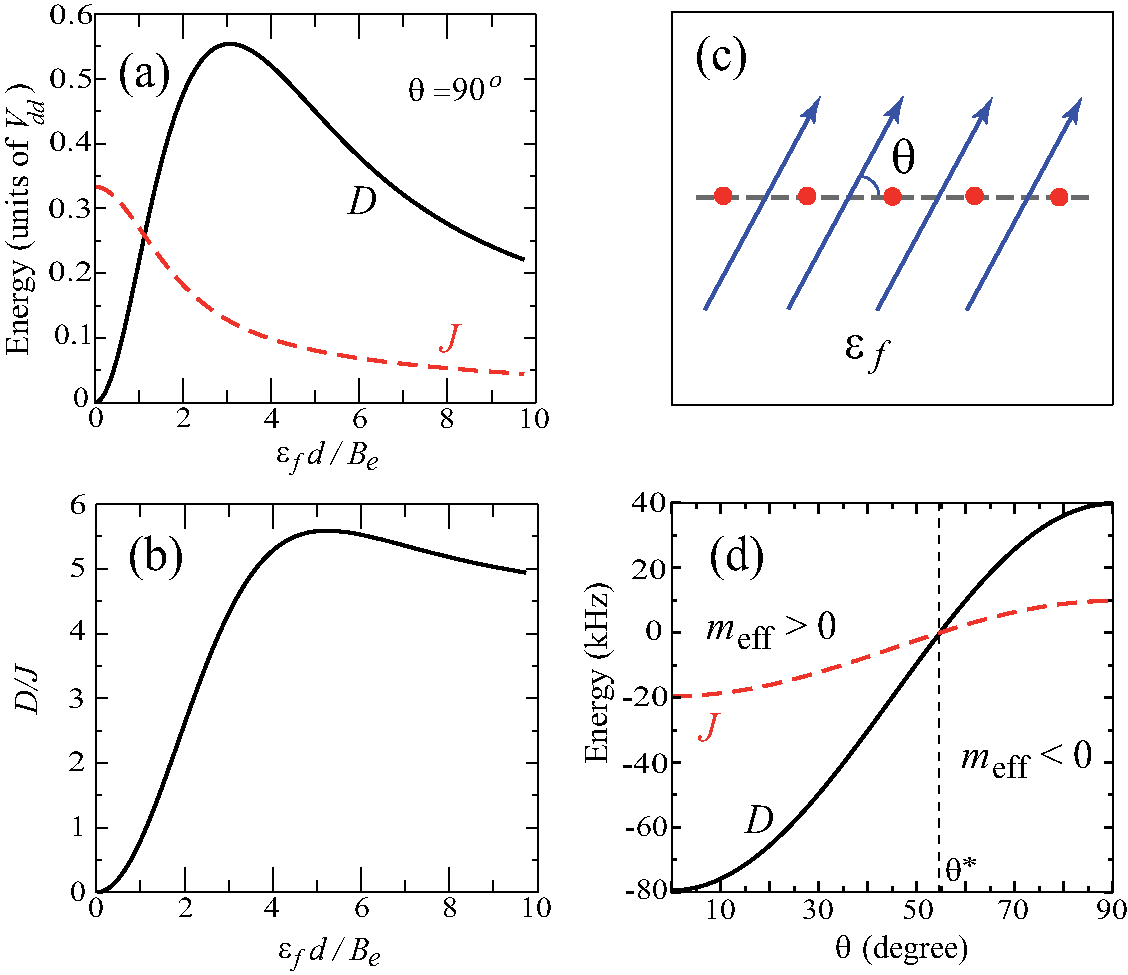
\includegraphics[scale=0.3]{Figure1FourPanels.pdf}
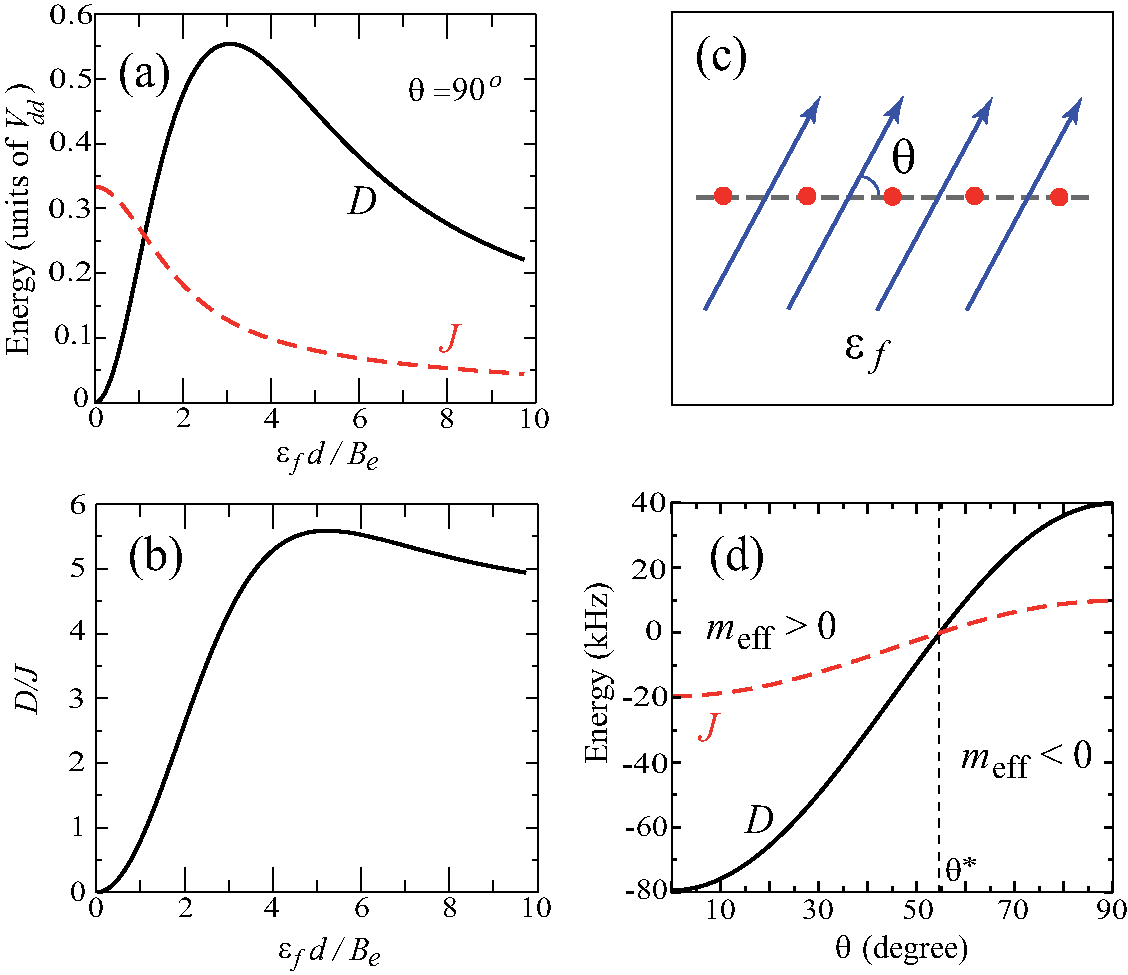
\includegraphics[width=\linewidth]{Figure1FourPanels.pdf}
\caption{ (a) The parameters $D$ and $J$ (in units of $V_{dd} = d^2/a^3$) as functions of the electric field strength.
 (b) The ratio  $D/J$ as a function of the electric field strength. The field is perpendicular to the intermolecular axis.
For LiCs molecules possessing the dipole moment $d$=5.529~Debye, the value ${\cal E}_f d/B_e = 1$ corresponds to
 ${\cal E}_f = 2.12$ kV/cm. (c) Schematic depiction of the angle $\theta$ between the field (represented by blue
 arrows) and the molecular array (represented by red dots). (d) $D$ and $J$ for a 1D array of LiCs molecules separated
 by 400 nm as functions of $\theta$ for ${\cal E}_f = 6$ kV/cm.
} \label{fig:HowDJChanges}
\end{figure}


\begin{figure}[htbp]
\centering
%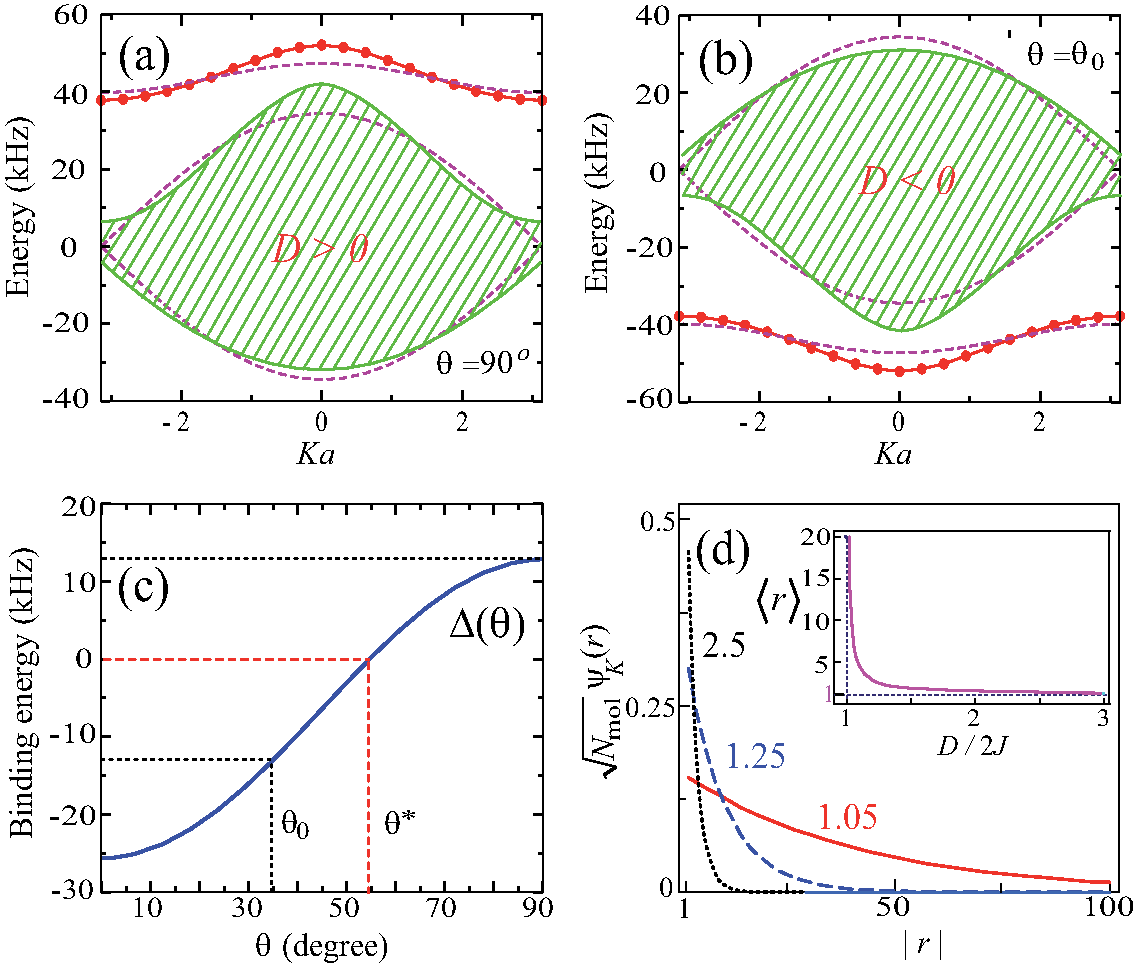
\includegraphics[scale=0.3]{FigureBiexciton.pdf}
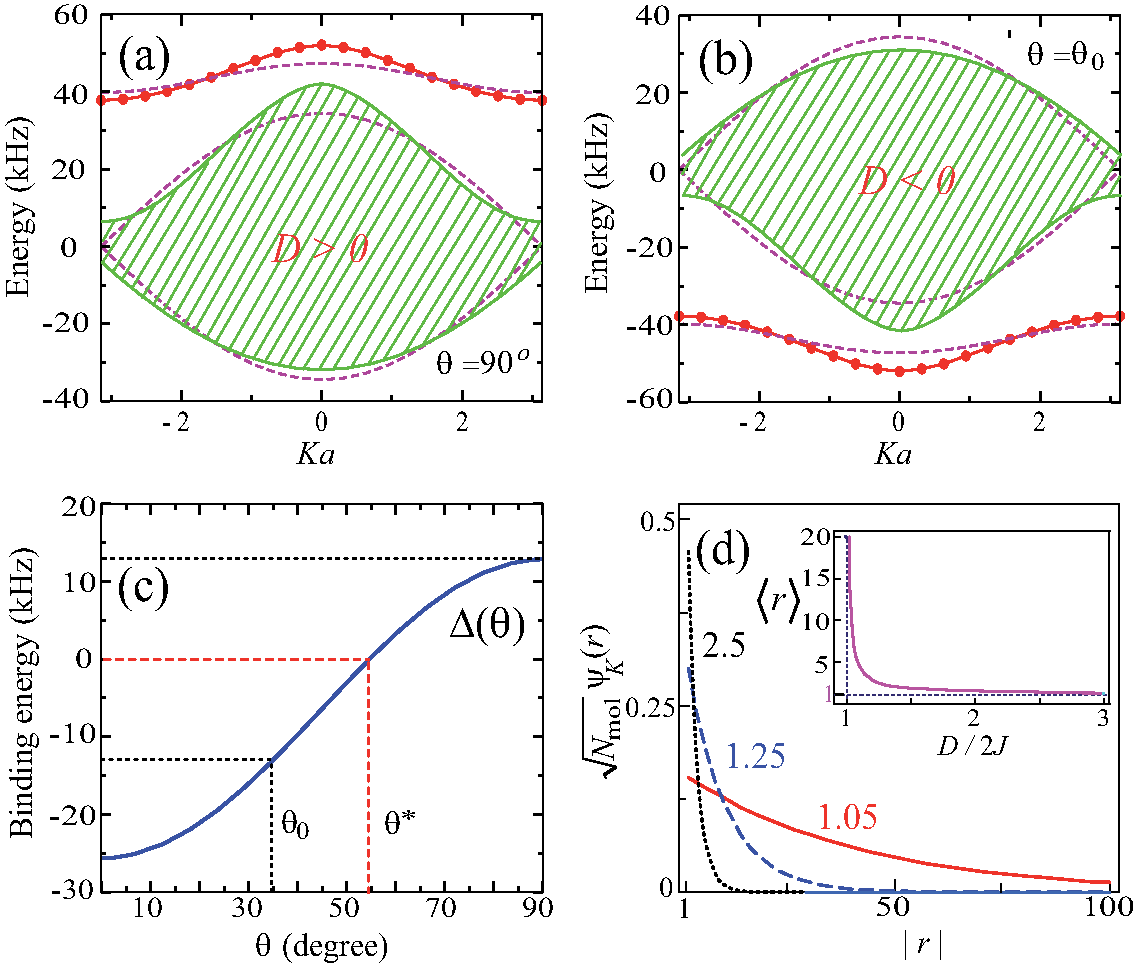
\includegraphics[width=\linewidth]{FigureBiexciton.pdf}
\caption{(a) and (b): Two-excitation spectra of a 1D array of LiCs molecules on an optical lattice: NNA
(dashed lines) and exact solutions (solid lines). The shaded regions encapsulate the bands of the continuum 
two-exciton states. (c)$\theta$-dependence of the biexciton binding energy $\Delta$. The electric field magnitude is
 6.88 kV/cm, $\theta_0 = \arccos \sqrt{2/3}$, $\theta^\ast = \arccos \sqrt{1/3}$. (d) Biexciton wave function vs the
 lattice site separation $|r|=|n-m|$ of the two excitations for $K=0$. Inset: Mean width of the biexciton wave function
 $\langle r \rangle$ calculated as the width of $\psi^{2}_{K}(r)$ at half maximum. Numbers at each curve indicate the
 value of $D/2J$.}
\label{fig:biexcitonSpectrum}
\end{figure}


For molecules in an optical lattice, the magnitudes of $J$ and $D$ depend on the strength of the applied electric field
 and the angle between the field and the molecular array  ($\theta$) (see \autoref{fig:HowDJChanges} (c) ).  We
 calculate these parameters for a 1D array of $^1\Sigma$ polar molecules (such as alkali metal dimers produced in
 ultracold molecule experiments) trapped on an optical lattice with the lattice separation $a = 400$ nm.
 \Autoref{fig:HowDJChanges} (b)
 shows that for a fixed angle $\theta$ the ratio $D/J$ increases as the electric field magnitude increases. 
For LiCs molecules, the condition (\ref{biexc-formation}) is satisfied for electric fields $>3.6$~kV/cm. Note that the
 ratio $D/J$ is independent of $\theta$. 

 Frenkel excitons are quasiparticles characterized by an effective mass ($m_{\rm eff}$). The sign of $J$ determines the
 sign of the  effective mass \cite{felipe}: negative $J$ corresponds to positive $m_{\rm eff}$ and vice versa (see
 \autoref{fig:HowDJChanges} (d) ). Due to the linearity of the Schr\"{o}dinger equation, a positive potential is
 attractive for particles with negative mass, just like a negative potential is attractive for particles with positive mass. 
 Because the sign of $J$ and $D$ is the same (and consequently the signs of $D$ and $m_{\rm eff}$ are opposite), the
 dynamical interaction (\ref{dynamical}) between excitons in this system is attractive.


To demonstrate the formation of the biexciton and calculate the biexciton energy, we diagonalize the Hamiltonian
 $\hat{H}_{\rm exc} + \hat{H}_{\rm dyn}$ for a one-dimensional array of $N_{\rm mol} = 501$ LiCs molecules. The
 matrix of the Hamiltonian is evaluated by expanding the biexciton states as 
\begin{eqnarray}
| \Psi_b(K) \rangle &=& \sum_{\substack{k_1 + k_2 = K \\ k_1 \ge k_2}} C_{k_1, k_2} \ket{k_1, k_2} \nonumber \\
&=&\sum\limits_{k \geq 0} C_k^K \ 
| \hat{P}^\dag(K/2 + k)  \hat{P}^\dag(K/2
- k) \rangle,
\label{wave-function} 
\end{eqnarray}
where $K = k_1+k_2$ and $k = (k_1 - k_2)/2$, and $k_1$ and $k_2$ denote the wavevectors of the interacting
 excitons. The Hamiltonian matrix is diagonalized numerically for fixed values of $K$, which is conserved.
 \Autoref{fig:biexcitonSpectrum} shows that for $\theta = 90^o > \theta^*=\arccos(1/\sqrt{3})$ the biexciton energy is
 above the two-exciton continuum (binding for particles with negative mass), and for
 $\theta = \arccos \sqrt{2/3} <  \theta^*$ below it (binding for particles with positive mass). The binding energy of the
 biexciton changes sign at $\theta = \theta^*$. The biexciton wave function $\psi_{K}(r)$ is plotted in
 \autoref{fig:biexcitonSpectrum} (d). \Autoref{fig:HowDJChanges} and \autoref{fig:biexcitonSpectrum} thus illustrate
 that the biexciton binding energy and size can be tuned by varying the strength and orientation of the electric field. 
 


\section{Non-optical creation of biexcitons} 
The possibility of formation of Frenkel biexcitons has been proposed quite long ago \cite{efremov1973}. However, in 
contrast to the well-known Wannier-Mott biexcitons in semiconductors, Frenkel biexcitons in solid-state molecular
 crystal are very difficult to observe. 
We now explain the reasons. First, many molecular crystals, such as anthracene or naphthalene,  possess inversion
 symmetry. In these crystals, the constant $D$ as defined in the line after \autoref{dynamical} must vanish and 
\autoref{biexc-formation} is not satisfied. Second, it is difficult to excite biexciton states optically: it was shown
 in Ref.\cite{Ezaki1994} that the oscillator strength for the photon-induced transitions to the biexciton state must
 decrease with the increasing binding energy of the biexcitons. Therefore, two-photon excitation can only produce
 unstable weakly bound biexcitons. Third, excitons in molecular crystals decay via bimolecular annihilation processes
 into higher-energy states and subsequent relaxation accompanied by emission of phonons. This process is prohibited
 by conservation of energy in an optical lattice with diatomic molecules. \Autoref{fig:HowDJChanges}  demonstrates
 that the first obstacle can be removed by tuning 
the electric field. To overcome the second obstacle, we propose a non-optical method of populating deeply bound
 biexciton states based on the unique structure of $^1\Sigma$ polar molecules. 
As zero electric field the rotational states $|g\rangle$ and $|e\rangle$ are separated by the energy 
$\Delta \epsilon_{e - g}= 2 B_e$, while the energy separation between state $|e\rangle$ and the next rotationally
 excited state $|f\rangle \equiv |N=2, M_N = 0\rangle$ is equal to $\Delta \epsilon_{e- f}=4B_e$. As the electric field
 increases, $\Delta \epsilon_{e - g}$ increases faster than $\Delta \epsilon_{e - f}$ (see \autoref{fig:rotationalEnergy}).
When ${\cal E}_f d/B_e \simeq 3.24$ (corresponding to ${\cal E}_f \simeq 6.88$ kV/cm for LiCs), 
$\Delta \epsilon_{f - g} = 2 \Delta \epsilon_{e - g}$. At electric fields near this magnitude, two 
$| g \rangle \rightarrow | e \rangle$ excitons can undergo the transition to the $|f \rangle$ state, and, inversely, 
the $|g \rangle \rightarrow |f\rangle$ excitation can produce a pair of $|g\rangle \rightarrow |e \rangle$ excitons or a
 biexciton state depicted in \autoref{fig:biexcitonSpectrum}. The coupling between states $| e \rangle$ and $| f \rangle$ is
$\hat{H}_{12} = \sum\limits_{n \neq m} M(n-m) \hat{R}_n  \hat{P}_n^\dag
\hat{P}_m^\dag$, where $M(n-m) = \langle e_{n},e_{m} | V_{dd}(n-m) | f_{n},g_{m}
\rangle$, and the operator $\hat{R}_n$ annihilates the $| f \rangle$
excitation in lattice site $n$. The total Hamiltonian describing this three-level 
system is $\hat{H}_{g-e-f} = \hat{H}_{\rm exc} + \hat{H}_{\rm dyn} +  \hat{H}_2 + \hat{H}_{12}$, where
$\hat{H}_2 = E_f \sum\limits_n \hat{R}_n^\dag \hat{R}_n   + \sum\limits_{n,m \neq n} J_{g-f}(n-m) \hat{R}_n^\dag \hat{R}_m $ and $J_{g-f}(n-m) = \langle g_{n},f_{m} | V_{dd}(n-m) | f_{n},g_{m} \rangle$.

\begin{figure}[htbp]
\centering
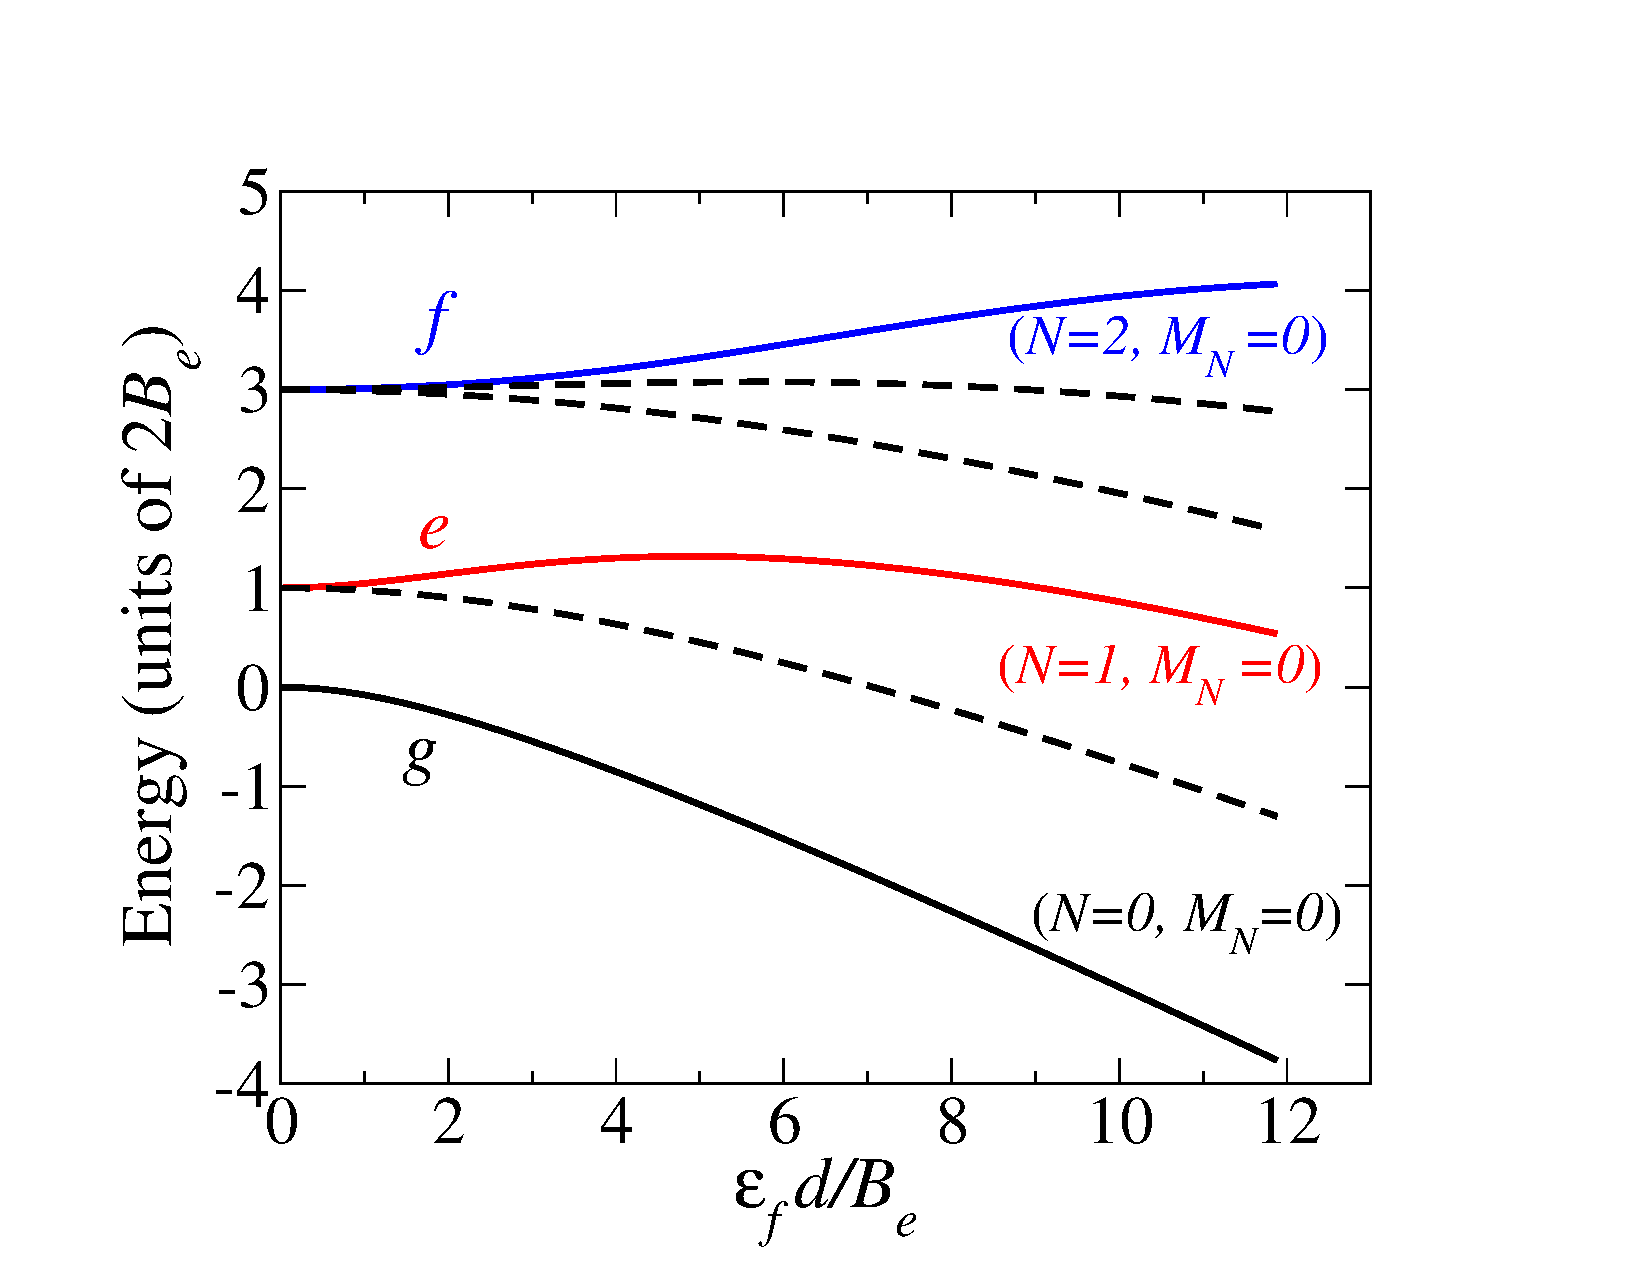
\includegraphics[width=\linewidth]{Figure3.pdf}
\caption{The rotational energies of a closed-shell polar molecule as functions of the strength of the DC field. The
 dashed lines represent other rotational states with $M_{N} \neq 0$. 
}
\label{fig:rotationalEnergy}
\end{figure}

\begin{figure}[htbp]
\centering
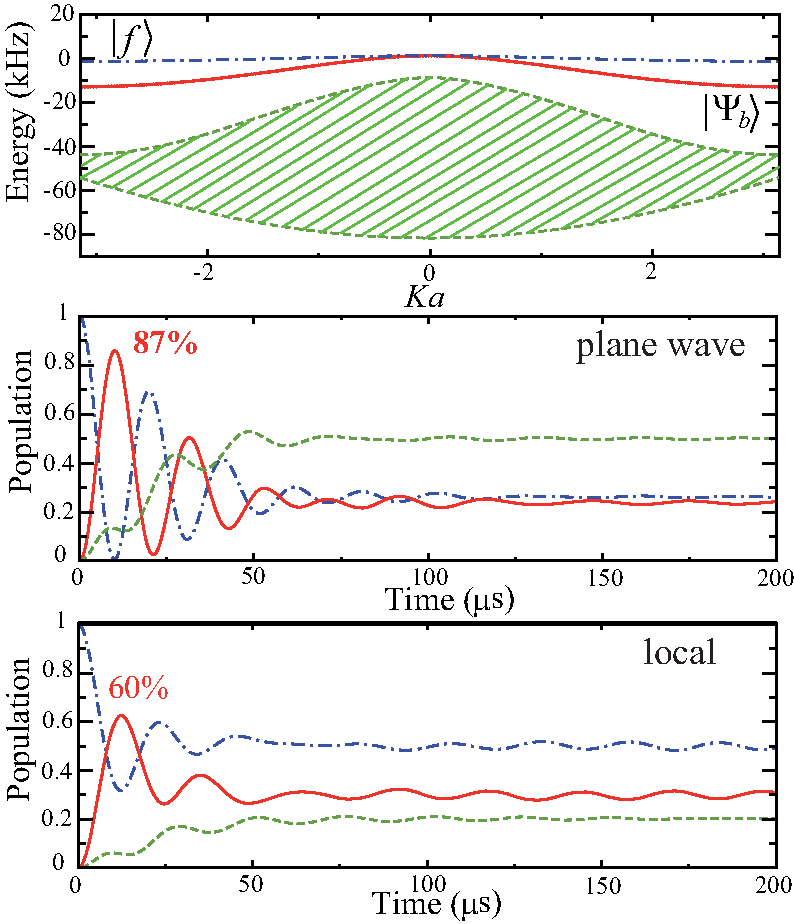
\includegraphics[scale=0.8]{Figure4.pdf}
%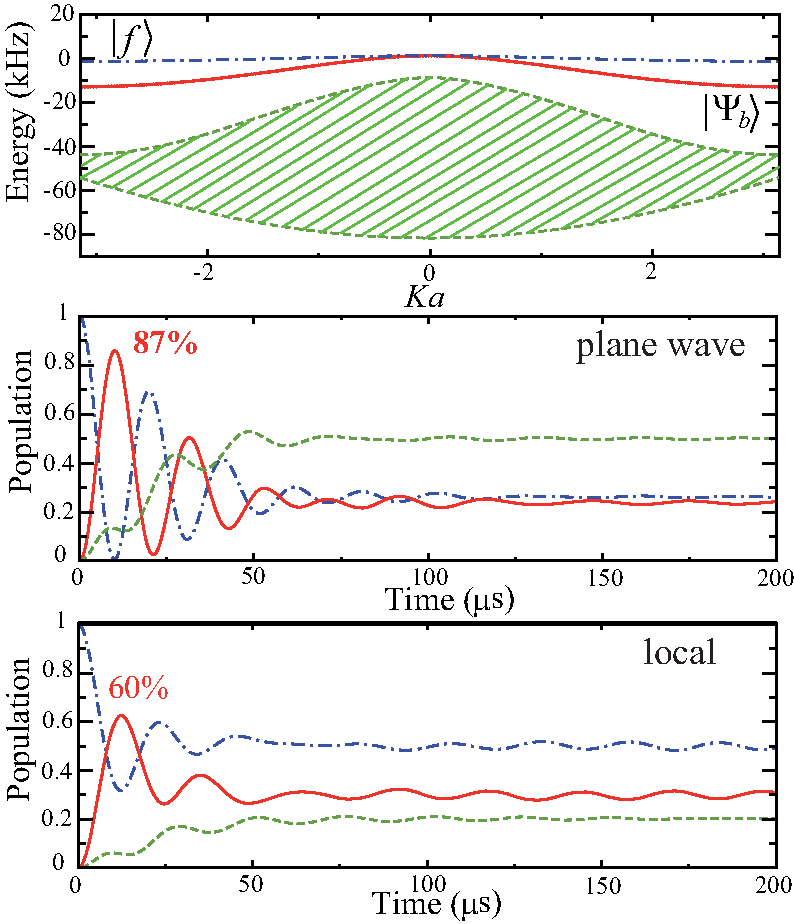
\includegraphics[width=\linewidth]{Figure4.pdf}
\caption{Population dynamics for the transition from $|g\rangle \to |f\rangle$ exciton (middle panel) and from an $f$
 state localized on a single molecule (lower panel) to coherent $|g\rangle \to |e\rangle$ excitons and biexcitons. The
 green dashed curves denote the population accumulated in the pairs of non-bound $|g\rangle \to |e\rangle$ exciton
 states, the red solid curves the biexciton state and the blue dot-dashed curves the $f$ state. The shaded region in the
 upper panel encapsulates the band of the continuum two-exciton states. The calculation is for a 1D ensemble of
 $N_{mol}=501$ LiCs molecules on an optical lattice with lattice separation a = 400 nm. The electric field of magnitude
 6.88 kV/cm is perpendicular to the molecular array.}
\label{fig:populationDynamics}
\end{figure}



In order to calculate the probability of the population transfer from state $f$ to the biexciton state, we solve the
 time-dependent Schr\"{o}dinger equation with the Hamiltonian $\hat{H}_{g-e-f}$ evaluated in the basis of products of
 the eigenstates of $\hat{H}_{\rm exc} + \hat{H}_{\rm dyn}$ and the eigenstates of $\hat{H}_2$. This leads to coupled
 differential equations:
\oneline{
i\hbar\mathbf{\dot{C}} = \mathbf{H}\mathbf{C} \ , \label{eqn:matrixDifferentialEqs}
} 
where $\mathbf{C}$ is a vector that represents a wavefunction in the basis set and $\mathbf{\dot{C}}$ is its derivative
with respect to time. Since the total Hamiltonian $\mathbf{H}$ is time-independent, we can make a basis-set 
transformation to diagonalize $\mathbf{H}$
\oneline{
\mathbf{U^{T}} \mathbf{H} \mathbf{U} = \mathbf{D} \ , 
}
 so that $\mathbf{C}$ in the new basis set can then be solved by direct
 integration and then $\mathbf{C}$ in the original basis set can be found by the inverse basis-set transformation. 
Multiplying both sides of \autoref{eqn:matrixDifferentialEqs}  by $\mathbf{U^{T}}$, we obtain
\multiline{
i\hbar\mathbf{U^{T}} \mathbf{\dot{C}} &=& \mathbf{U^{T}} \mathbf{H} \mathbf{U} \mathbf{U^{T}}\mathbf{C} \ , \label{eqn:matrixDifferentialEqsModified}
}
where $ \mathbf{U} \mathbf{U^{T}} = \mathbf{I}$ has been used. Let's define
\oneline{
\mathbf{A} \equiv \mathbf{U^{T}} \mathbf{C} \ , \label{eqn:changeBasis}
}
then
\oneline{
\mathbf{\dot{A}} =  \mathbf{U^{T}} \mathbf{\dot{C}} 
}
because $\mathbf{H}$ is time-independent and $\mathbf{U^{T}}$ must be time-independent too.  
So \autoref{eqn:matrixDifferentialEqs} can be rewritten as
\oneline{
i\hbar \mathbf{\dot{A}} = \mathbf{D} \mathbf{A} \ , 
}
which can solved easily by direct integration:
\oneline{
\mathbf{A}(t) = e^{-\frac{i}{\hbar} \mathbf{D} \; t} \mathbf{A}(0) \ .  \label{eqn:solForA}
}
Substituting \autoref{eqn:changeBasis} into \autoref{eqn:solForA}, we get
\oneline{
\mathbf{C}(t) = \mathbf{U} e^{-\frac{i}{\hbar} \mathbf{D} \; t} \mathbf{U^{T}} \mathbf{C}(0) \ ,  \label{eqn:solForC}
}
where $\mathbf{D}$ is a diagonal matrix whose non-zero elements are the eigenvalues of $\mathbf{H}$, and each
column of $\mathbf{U}$ is an eigenvector of $\mathbf{H}$. Therefore, given the eigenvalues and eigenvectors of the
total Hamiltonian and the initial wavefunction $\mathbf{C}(0)$, the wavefunction $\mathbf{C}(t)$ at any time $t$ can
be calculated from \autoref{eqn:solForC}. In our numerical calculations, we use subroutines from the LAPACK library
to calculate the eigenvalues and eigenvectors of the matrix. 


The magnitude of $J_{g-f}$ is about ten times smaller than $J$.
 In the absence of decoherence, the $| g \rangle \rightarrow | f \rangle$ excitation gives rise to the Frenkel exciton and
 the transition from the $f$ states to 
 the biexciton state is a coherent exciton--exciton transition. In the presence of decoherence, the exciton states
 become localized. If the decoherence rate is larger than $J_{g-f}/h$, but smaller than $J/h$, the
 $| g \rangle \rightarrow | f \rangle$ excitation is localized, while the biexciton states remain coherent.
 \Autoref{fig:populationDynamics} presents the calculations of the population transfer probabilities for both
 scenarios. The results show that the biexciton states can be populated with high efficiency. The equilibrium
 populations (in the limit of large $t$) depend on the relative energies of the $f$ state, the biexciton bound state and
 exciton--exciton continuum states, which can be tuned by varying the electric field magnitude. 
The efficiency of the population transfer can be maximized if the electric field is detuned far away from resonance
 when the biexciton population oscillations reach the first maximum. Detuning the electric field to low magnitudes
 effectively decouples the $f$ state from the states in the $\{g,e\}$ subspace and interrupts the population dynamics.
 This corresponds to switching off the channel for bimolecular annihilation of excitons, which is one of the reasons of
 the biexciton population depletion in solids. We have confirmed that the calculations with electric fields $< 5.0$
 kV/cm yield no  noticeable population transfer. 

\section{Extension to exciton trimers}
\label{sec:trimers}
In \autoref{sec:biexciton}, it is shown that Frenkel rotational biexcitons exist under some conditions in optical lattices. 
Then the question arises naturally: if two excitons can bind together, what about three excitons? In this section, we
extend the method to handle the three-exciton case and answer the question about exciton trimers. 

Similar to the case of biexciton, we define a three-exciton wavefunction in site representation
\oneline{
\ket{\Psi} = \sum_{n_1, n_2, n_3} C_{n_1, n_2, n_3}\pd{n_1}\pd{n_2}\pd{n_3} \ket{0} \ , 
}
and start from the Sch{\"o}dinger equation with the same Hamiltonian 
$\hat{H} = \hat{H}_{\rm exc} + \hat{H}_{\rm dyn} $
\oneline{
\hat{H} \ket{\Psi} = E_{\rm trimer}  \ket{\Psi}  \ . \label{eqn:schrodingerTrimer}
}
Since two excitations can't sit at the same molecule, we have the constraint on $C_{n_1, n_2, n_3}$:
\oneline{
C_{n_1, n_2, n_3} = 0 \;\; \mbox{\rm if $n_1 = n_2$ or $n_2 = n_3$ or $n_1 = n_3$} \ . \label{eqn:trimerConstraint}
} 
After similar derivations as we did for the biexciton case, \autoref{eqn:schrodingerTrimer} and
 \autoref{eqn:trimerConstraint} lead to
\multiline{
&&\left[3 E _0 D(n_1-n_2) + D(n_1-n_3) + D(n_2 - n_3) - E_{\rm trimer} \right] C_{n_1, n_2, n_3} \nonumber \\
&& \hspace{0.5cm} + \sum _n\left[J(n- n_1)C_{n, n_2, n_3} + J(n-n_2)C_{n_1, n, n_3} + J(n-n_3 )C_{n_1, n_2, n}\right] \nonumber \\
&& = 2\delta _{n_1,n_2}\sum _{n}J(n_1-n)C_{n, n_2, n_3} + 2\delta _{n_2, n_3}\sum _{n}J(n_2 -n)C_{n_1, n, n_3} \nonumber \\
&&  \hspace{0.5cm} + 2\delta _{n_1,n_3}\sum _{n} J(n_3 -n)C_{n_1, n_2, n}  \ . \nonumber \\ \label{eqn:schrodingerTrimerSite}
}
Note that the equation can't be used to determine the values of $C_{n_1, n_2, n_3}$ when any two of $n_1$, $n_2$, and $n_3$ are equal. Using the following Fourier transform
\oneline{
C_{n_1, n_2, n_3} = \frac{1}{\left(\sqrt{N_{\rm mol}}\right)^3}\sum_{k_1, k_2, k_3} C(k_1, k_2, k_3) e^{i (k_1 n_1 + k_2 n_2 + k_3 n_3) }
}
we can transform \autoref{eqn:schrodingerTrimerSite} to 
\multiline{
&&\frac{1}{N_{\rm mol}}\sum _{q}\Tilde{D}(q) \left[C(k_1-q, k_2+q, k_3)+C(k_1 -q, k_2, k_3+q)+C(k_1,k_2-q,k_3+q)\right] \nonumber \\
&& \hspace{0.5cm} + \left[\epsilon(k_1)+ \epsilon(k_2)+ \epsilon(k_3)-E _{\rm trimer}\right]C(k_1, k_2, k_3) \nonumber \\ 
&&=\frac{2}{N_{\rm mol}}\sum _{q}\left[ \Tilde{J}(k_1-q)C(k_1-q,k_2+q,k_3)+\Tilde{J}(k_2-q)C(k_1,k_2-q,k_3+q) \right. \nonumber \\
&& \left.  \hspace{1.5cm} + \Tilde{J}(k_3-q)C(k_1+q,k_2+q,k_3-q)\right] \ , \label{eqn:threeBodyEq}
}
which can be written as an eigenvalue problem
\oneline{
\sum_{k_1^{'} + k_2^{'} + k_3^{'} = K} \mathbf{A}_{k_1 k_2 k_3; k_1^{'} k_2^{'} k_3^{'}} C(k_1^{'}, k_2^{'}, k_3^{'}) = E _{\rm trimer} C(k_1, k_2, k_3) \ , \label{eqn:trimerMatrixEq}
} 
where 
\multiline{
\mathbf{A}_{k_1 k_2 k_3; k_1^{'} k_2^{'} k_3^{'}} &=& \delta_{k_1, k_1^{'}} \delta_{k_2, k_2^{'}} \delta_{k_3, k_3^{'}} \left[ \epsilon(k_1) + \epsilon(k_2) + \epsilon(k_3)\right]  \nonumber \\
&& + \frac{1}{N_{\rm mol}} \left\{ \delta_{k_1, k_1^{'}} \left[ \Tilde{D}(k_2 - k_2^{'}) -2 \Tilde{J}(k_2^{'})  \right] \right. \nonumber \\
&&\hspace{1.5cm} +  \delta_{k_2, k_2^{'}} \left[ \Tilde{D}(k_3 - k_3^{'}) -2 \Tilde{J}(k_3^{'})  \right] \nonumber \\
&&\hspace{1.5cm} \left. +  \delta_{k_3, k_3^{'}} \left[ \Tilde{D}(k_1 - k_1^{'}) -2 \Tilde{J}(k_1^{'})  \right] \right\} \ .
}
The above equations clearly show that only those coefficients $C(k_1, k_2, k_3)$ whose wavevectors add up to a fixed $K$
 are coupled to each other. Therefore, the eigenvalues for each value of $K$ can be calculated independently.
However, since we assumed that $C_{n_1, n_2, n_3} = 0$
when any two of $n_1, n_2, n_3$ are equal, we need to take care of the constraint when solving
 \autoref{eqn:trimerMatrixEq}. 

Let's examine the effect of  the constraint on $C_{n_1, n_2, n_3}$. Assuming $k_3$ is fixed, we have
\multiline{
\sum_{k_1 + k_2 = K - k_3} C(k_1, k_2, k_3) &=& \sum_{k_1}\sum_{n_1, n_2, n_3 }\frac{1}{\left( \sqrt{N_{\rm mol}}\right)^3} e^{i (k_1 n_1 + k_2 n_2 + k_3 n_3 )} C_{n_1, n_2, n_3} \nonumber \\
&=& \sum_{n_1, n_2, n_3 }\frac{1}{ \sqrt{N_{\rm mol}}} \left( \frac{1}{N_{\rm mol}}\sum_{k_1}e^{i k_1 (n_1 - n_2) }\right) e^{i (K - k_3 ) n_2} e^{i k_3 n_3} C_{n_1, n_2, n_3} \nonumber \\
&=&\sum_{n_1, n_2, n_3 }\frac{1}{ \sqrt{N_{\rm mol}}}  \delta_{n_1, n_2} e^{i (K - k_3 ) n_2} e^{i k_3 n_3} C_{n_1, n_2, n_3} \nonumber \\
&=&\sum_{ n_2, n_3 }\frac{1}{ \sqrt{N_{\rm mol}}} e^{i (K - k_3 ) n_2} e^{i k_3 n_3} C_{n_2, n_2, n_3} \nonumber \\
&=& 0 \ . \label{eqn:specificCondition}
}


Since the fixed wavector $k_3$ can be chosen arbitrarily, a condition similar to  \autoref{eqn:specificCondition} will
hold for a fixed $k_1$ and a fixed $k_2$ as well. This means:  for a particular $K$ if you add up all  
$C(k_1^{'}, k_2^{'}, k_3^{'})$ whose first (second or third) wavevector $k_1^{'} ( k_2^{'} \mbox{ or }  k_3^{'})$ equal to a fixed $k$, you will get zero. Thus we can add the zero
\multiline{
&&\frac{1}{N_{\rm mol}} \sum_{k_1^{'}, k_2^{'}, k_3^{'} } \left[ -2\Tilde{J}(k_2) \delta_{k_1^{'}, k_1} C(k_1^{'}, k_2^{'}, k_3^{'})  -2\Tilde{J}(k_3) \delta_{k_2^{'}, k_2} C(k_1^{'}, k_2^{'}, k_3^{'}) \right. \nonumber \\
&& \left. -2\Tilde{J}(k_1) \delta_{k_3^{'}, k_3} C(k_1^{'}, k_2^{'}, k_3^{'}) \right] = 0
}
 to the left hand side of \autoref{eqn:trimerMatrixEq} to produce a new equation
\oneline{
\sum_{k_1^{'} + k_2^{'} + k_3^{'} = K} \mathbf{B}_{k_1 k_2 k_3; k_1^{'} k_2^{'} k_3^{'}} C(k_1^{'}, k_2^{'}, k_3^{'}) = E _{\rm trimer} C(k_1, k_2, k_3) \ , \label{eqn:trimerMatrixEqSymmetric}
} 
where
\multiline{
\mathbf{B}_{k_1 k_2 k_3; k_1^{'} k_2^{'} k_3^{'}} &=& \delta_{k_1, k_1^{'}} \delta_{k_2, k_2^{'}} \delta_{k_3, k_3^{'}} \left[ \epsilon(k_1) + \epsilon(k_2) + \epsilon(k_3)\right]  \nonumber \\
&& + \frac{1}{N_{\rm mol}} \left\{ \delta_{k_1, k_1^{'}} \left[ \Tilde{D}(k_2 - k_2^{'}) -2 \Tilde{J}(k_2) -2 \Tilde{J}(k_2^{'})  \right] \right. \nonumber \\
&&\hspace{1.5cm} +  \delta_{k_2, k_2^{'}} \left[ \Tilde{D}(k_3 - k_3^{'}) -2 \Tilde{J}(k_3) -2 \Tilde{J}(k_3^{'})  \right] \nonumber \\
&&\hspace{1.5cm} \left. +  \delta_{k_3, k_3^{'}} \left[ \Tilde{D}(k_1 - k_1^{'}) -2 \Tilde{J}(k_1)-2 \Tilde{J}(k_1^{'})  \right] \right\} \ .
}
The advantage of \autoref{eqn:trimerMatrixEqSymmetric} over \autoref{eqn:trimerMatrixEq} is that the matrix
$\mathbf{B}$ is symmetric, which leads to easier diagonalization. 

The energies of three-exciton states can be obtained by diagonalizing the matrix $\mathbf{B}$ in
 \autoref{eqn:trimerMatrixEqSymmetric} and filtering out the eigenvalues whose corresponding eigenvectors don't
 satisfiy \autoref{eqn:specificCondition}. As a proof-of-principle example, we have solved
 \autoref{eqn:trimerMatrixEqSymmetric} for a small lattices under the nearest-neighbor approximation and presented
 the results  in \autoref{fig:trimer}. As can be seen from the figure, three excitons may
form a three-body bound state or a biexciton plus a free exciton. Since the energies of three-body bound states are
located outside the energy continuum of a biexciton plus a free exciton, an interesting question arise: does 
three-body bound states of excitons exist when two-body bound states don't form, that is, does the Efimov effect
 occur in the current case? Unfortunately, numerical investigation shows that the three-body and
 two-body bound states always occur at the same time when $D/J$ reaches 2, indicating no Efimov effect. However,
this is not a conclusive result as only the interaction between nearest neighbors are included in the calculation and 
the effect of long-range interaction need to be examined.

 

\begin{figure}[htbp]
\centering
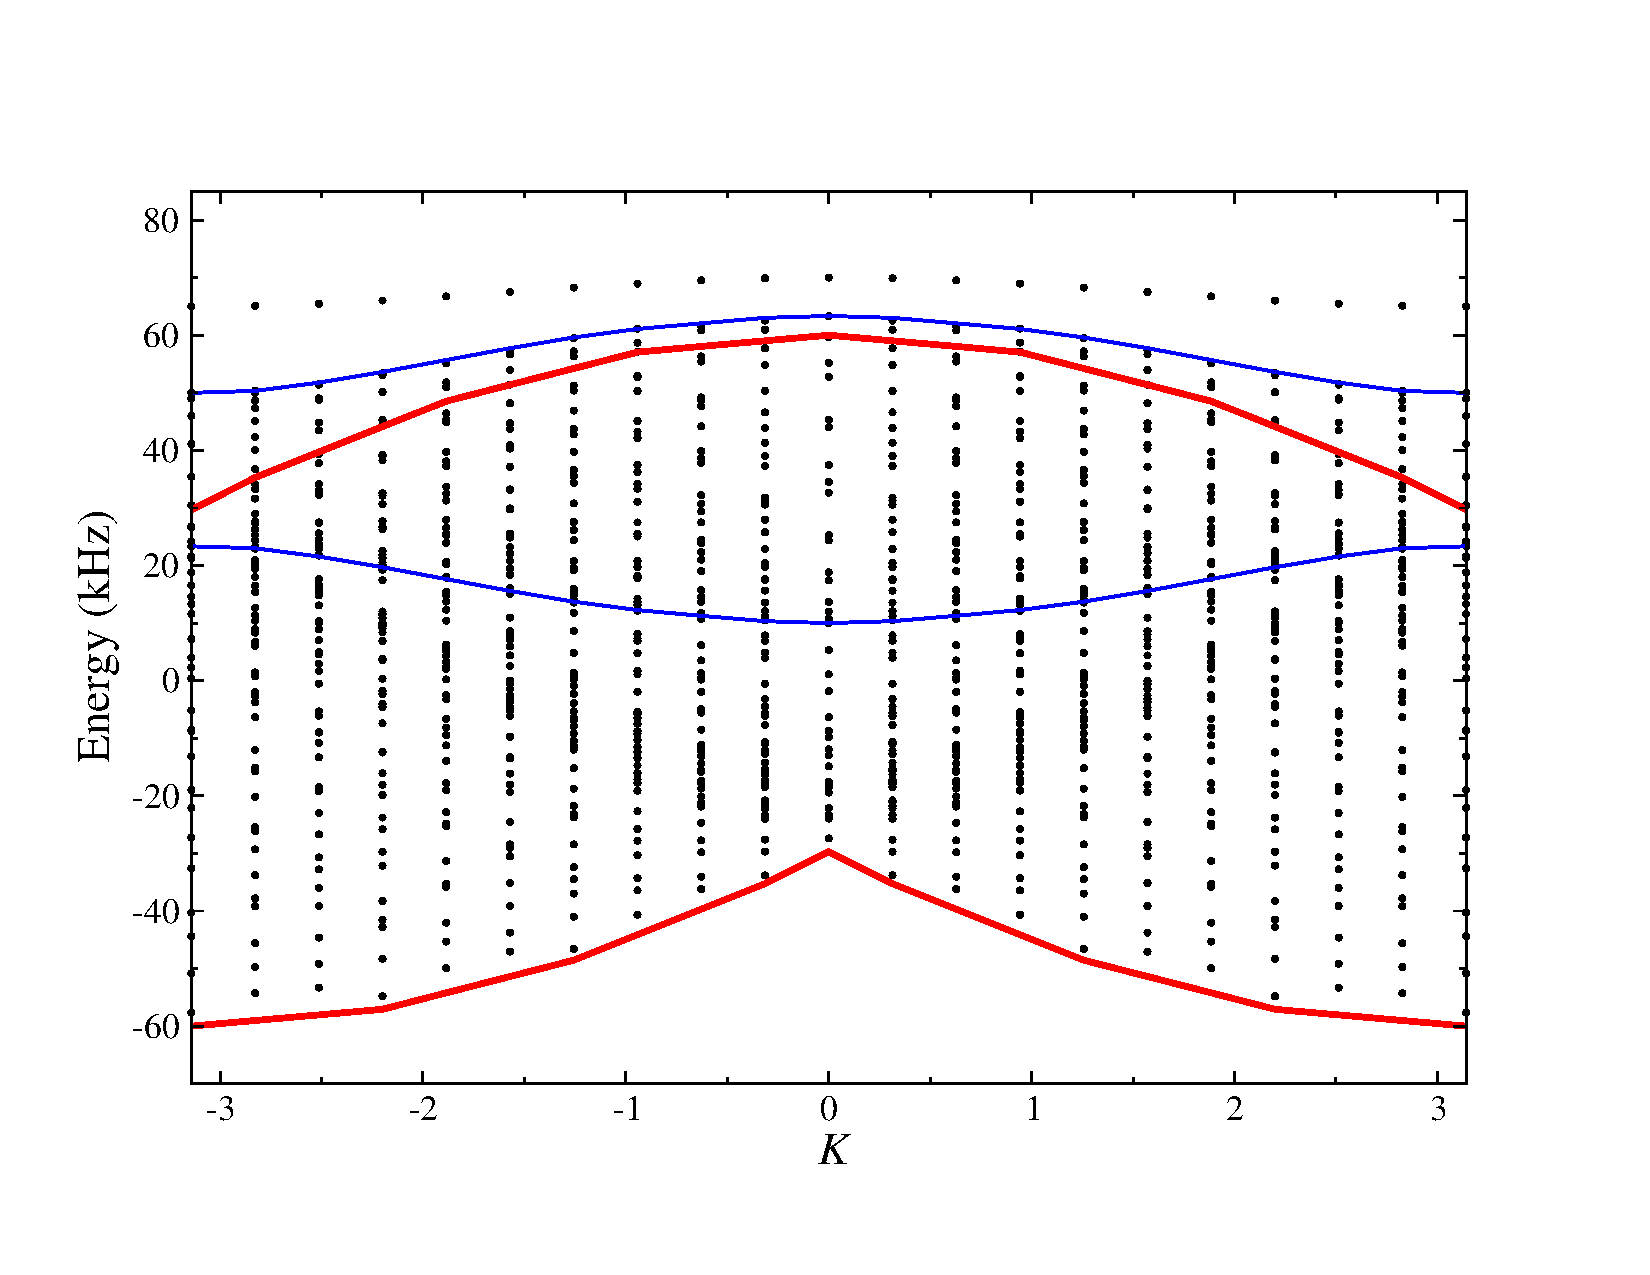
\includegraphics[width=\linewidth]{threeExcitons.pdf}
\caption{Three-excitation spectra of a 1D array of molecules on an optical lattice. The calculation is done for a
 system of 20 lattice sites with the hopping interaction $J =10$ kHz and the dynamic interaction $D =30$ kHz.
The black dots represent energies of all three-exciton states, the red curves denote the boundaries of  energy
 continuum of three free excitons, and the blue curves represent the boundaries of energy continuum for a biexciton 
plus a free exciton. 
   }
\label{fig:trimer}
\end{figure}


\section{Discussion} 
We have shown that rotational excitation of molecules trapped on an optical lattice gives rise to rotational excitons
 whose interactions can be controlled by an external electric field. The exciton--exciton interactions can be tuned to
 produce two-exciton bound states.  A biexciton is an entangled state of two Frenkel excitons. The creation of
 biexcitons as described in the previous section and tuning the electric field to the regime of zero binding energy can
 thus be used for the controlled preparation of entangled pairs of non-interacting excitons. In order to observe the
 biexcitons, one could measure correlations between the populations of the rotationally excited states of molecules in
 different lattice sites using the method proposed in Ref. \cite{demille}. 




The present work suggests several interesting questions. For example, it was recently shown that Frenkel excitons in
 shallow optical lattices can be coupled to lattice phonons, leading to polarons \cite{felipe-polarons}. Coupling a
 Frenkel biexciton to phonons would produce strongly interacting polarons. It would be interesting to explore if these
 interactions lead to the formation of bipolarons. 



We have repeated the calculations presented here for a system of three excitons and similarly observed the formation
 of three-exciton bound states. It would be interesting to explore the effect of tunable exciton--exciton interactions
 on excitation correlations, both as a function of $D/J$ and the density of excitations, to understand fundamental
 limits of exciton clustering \cite{exciton-cluster}. 


The creation of biexcitons with tunable binding energy and measuring quantum energy transport for different ratios
 $D/J$ can be used to study the effects of exciton--exciton entanglement on energy transfer in molecular aggregates
 \cite{photosynthesis-1,photosynthesis-2,photosynthesis-3}. The ability to tune exciton--exciton interactions can be
 used to explore the role of multiple excitation correlations on energy transfer in disordered systems (the confining
 lattice potential can be tilted or the molecules can be perturbed by a disorder potential produced by an
 inhomogeneous electric field).
  



